\documentclass{article}

\usepackage{microtype}
\usepackage{graphicx}
\usepackage{booktabs} %

\usepackage[breaklinks]{hyperref}

\newcommand{\theHalgorithm}{\arabic{algorithm}}

\usepackage[accepted]{icml2023}


\usepackage{amsmath}
\usepackage{amssymb}
\usepackage{mathtools}
\usepackage{amsthm}

\usepackage{url}
\usepackage[utf8]{inputenc} %
\usepackage[T1]{fontenc}    %
\usepackage[breaklinks]{hyperref}      %
\usepackage{url}            %
\def\UrlBreaks{\do\/\do-}
\usepackage{booktabs}       %
\usepackage{amsfonts}       %
\usepackage{amsmath}
\usepackage{amssymb}
\usepackage{mathtools}
\usepackage{amsthm}
\usepackage{nicefrac}       %
\usepackage{microtype}      %
\usepackage{xcolor}         %
\usepackage{wrapfig}
\usepackage{graphicx}
\usepackage{caption}
\usepackage{multirow,makecell}

\usepackage{xspace}
\usepackage{subcaption}
\newcommand{\algname}[1]{{\sc #1}\xspace}
\usepackage{algorithm}
\usepackage{algorithmic}

\newcommand{\newstuff}[1]{{\color{blue}#1}}

\usepackage[capitalize,noabbrev]{cleveref}

\theoremstyle{plain}
\newtheorem{theorem}{Theorem}[section]
\newtheorem{proposition}[theorem]{Proposition}
\newtheorem{lemma}[theorem]{Lemma}
\newtheorem{corollary}[theorem]{Corollary}
\theoremstyle{definition}
\newtheorem{definition}[theorem]{Definition}
\newtheorem{assumption}[theorem]{Assumption}
\theoremstyle{remark}
\newtheorem{remark}[theorem]{Remark}

\usepackage[textsize=tiny]{todonotes}


\icmltitlerunning{SWARM Parallelism: Training Large Models Can Be Surprisingly Communication-Efficient}

\begin{document}

\twocolumn[
\icmltitle{SWARM Parallelism: Training Large Models\\ Can Be Surprisingly Communication-Efficient}



\icmlsetsymbol{equal}{*}

\begin{icmlauthorlist}
\icmlauthor{Max Ryabinin}{equal,hse,yandex}
\icmlauthor{Tim Dettmers}{equal,uw}
\icmlauthor{Michael Diskin}{yandex,hse}
\icmlauthor{Alexander Borzunov}{hse,yandex}
\end{icmlauthorlist}

\icmlaffiliation{hse}{HSE University}
\icmlaffiliation{yandex}{Yandex}
\icmlaffiliation{uw}{University of Washington}

\icmlcorrespondingauthor{Max Ryabinin}{mryabinin0@gmail.com}

\icmlkeywords{Machine Learning, ICML}

\vskip 0.3in
]



\printAffiliationsAndNotice{\icmlEqualContribution} %

\begin{abstract}




Many deep learning applications benefit from using large models with billions of parameters. Training these models is notoriously expensive due to the need for specialized HPC clusters. In this work, we consider alternative setups for training large models: using cheap ``preemptible'' instances or pooling existing resources from multiple regions. We analyze the performance of existing model-parallel algorithms in these conditions and find configurations where \textit{training larger models becomes less communication-intensive}.
Based on these findings, we propose SWARM parallelism\footnote{SWARM parallelism is a backronym for Stochastically Wired Adaptively Rebalanced Model Parallelism.}, a model-parallel training algorithm designed for poorly connected, heterogeneous and unreliable devices. SWARM creates temporary randomized pipelines between nodes that are rebalanced in case of failure. 
We empirically validate our findings and compare SWARM parallelism with existing large-scale training approaches.
Finally, we combine our insights with compression strategies to train a large Transformer language model with 1B shared parameters (${\approx}13$B before sharing) on preemptible T4 GPUs with less than 200Mb/s network.





 
\end{abstract}

\section{Introduction}\label{sec:intro}
% Multi-armed bandit (MAB) is a classic sequential decision making problem \citep{auer2002finite}, where a learning agent chooses among competing actions sequentially to maximize its accumulative reward over time. 
% %Despite its simplicity, MAB exemplifies the exploration-and-exploitation dilemma that also exists in more complicated problems. 
% An important extension of MAB, named linear contextual bandit \citep{li2010contextual}, incorporates contextual information in the problem setting, by assuming a linear mapping between the context and expected reward. It has gained popularity in various applications, such as recommender systems \citep{li2010contextual}, display advertisement \citep{li2010exploitation} and clinical trials \citep{durand2018contextual}.
% Most existing linear bandit solutions are designed under a centralized learning setting, i.e., data is readily available at a central server. However, with the increasing public concerns of privacy, especially the bandit algorithms usually directly learn from user data,
% %more and more people are reluctant to provide their own data and strict regulations on data usage like GDPR have also went into effect \cite{voigt2017eu}, which makes 
% there is a growing demand to keep data decentralized and push the learning of bandit models to the client side. 
% % This idea is also made much more feasible due to the growing computational power of edge devices nowadays. 

% Federated learning has recently emerged as a promising setting for decentralized machine learning.
% % , and its effectiveness was first validated at a large scale by training a global model across all mobile devices via the Google Keyboard Android application \cite{konevcny2016federated}. 
% %The term ``federated learning" was first introduced by \citet{mcmahan2017communication} with an emphasis on efficiently training deep models over mobile device applications. As significant amount of later works have applied federated learning to other applications, there may be variations in its meaning for different research communities. 
% Since its debut in \citet{mcmahan2017communication}, there have been variations in its definition for different applications \citep{yang2019federated}.
% In this paper, we follow the general definition by \citet{kairouz2019advances}: multiple clients collaborate in solving a machine learning problem under the coordination of a central server, while keeping each client's raw data local. 
% So far, most existing works in federated learning study offline supervised learning problems \citep{konevcny2016federated,zhao2018federated}, where labeled training instances already sit on the client side. How to perform bandit learning under the federated learning setting remains underexplored.
As a popular online learning problem, linear contextual bandit has been used for a variety of applications, including recommender systems \citep{li2010contextual}, display advertisement \citep{li2010exploitation} and clinical trials \citep{durand2018contextual}. While most existing solutions are designed under a centralized setting (i.e., data is readily available at a central server), in response to the increasing application scale and public concerns of privacy, there is a growing demand to keep data decentralized and push the learning of bandit models to the client side.
% As a classic sequential decision making problem, linear contextual bandit has been widely used for a variety of real-world applications, including recommender systems \citep{li2010contextual}, display advertisement \citep{li2010exploitation} and clinical trials \citep{durand2018contextual}. 
% Most existing solutions are designed under a centralized learning setting, i.e., data is readily available at a central server. However, with the increasing public concerns of privacy, especially the bandit algorithms usually directly learn from user data,
% there is a growing demand to keep data decentralized and push the learning of bandit models to the client side. 
Federated learning has recently emerged as a promising setting for decentralized machine learning \citep{konevcny2016federated}.
% , and its effectiveness was first validated at a large scale by training a global model across all mobile devices via the Google Keyboard Android application \cite{konevcny2016federated}. 
%The term ``federated learning" was first introduced by \citet{mcmahan2017communication} with an emphasis on efficiently training deep models over mobile device applications. As significant amount of later works have applied federated learning to other applications, there may be variations in its meaning for different research communities. 
Since its debut in \citeyear{mcmahan2017communication}, there have been many variations for different applications \citep{yang2019federated}. However, most existing works study offline supervised learning problems \citep{li2019convergence,zhao2018federated}, which only concerns optimization convergence over a fixed dataset. How to perform federated bandit learning remains under-explored, and is the main focus of this paper. 

Analogous to its offline counterpart, the goal of federated bandit learning is to minimize the cumulative regret incurred by $N$ clients during their online interactions with the environment over time horizon $T$,
% $N$ clients in a learning system need to collaborate to minimize the overall cumulative regret over a finite time horizon $T$, 
while keeping each client's raw data local. Take recommender systems as an example, where the clients correspond to the edge devices that directly interact with user by making recommendations and receiving feedbacks. Unlike centralized setting where observations from all clients are immediately transmitted to the server to learn a single model, in federated bandit learning, each client makes recommendations based on its local model, with occasional communication for collaborative model estimation.

% In this paper, we follow the general definition by \citet{kairouz2019advances}: multiple clients collaborate in solving a machine learning problem under the coordination of a central server, while keeping each client's raw data local. 


%Though having potential for wide range of applications, online learning problems like linear bandit in federated learning setting, a.k.a. federated linear bandits \cite{dubey2020differentially}, have not attracted enough attention and still remain an open problem. 

% Therefore, it is a natural idea to study contextual linear bandit in a federated learning paradigm, which is also referred to as federated linear bandits \cite{dubey2020differentially}. In a federated learning paradigm, multiple clients collaborate in solving a machine learning problem, under the coordination of a central server, and each client's raw data is stored locally and not transferred to the server. 
% when linear bandit algorithms are applied to the federated learning paradigm, because these algorithms assume a traditional centralized machine learning system where all the data are collected together and all the computation happens in one machine or data center. 
Several new challenges arise in this problem setting. 
The first is the conflict between the need of timely data/model aggregation for \emph{regret minimization} and the need of \emph{communication efficiency}, since communication is the main bottleneck for many distributed application scenarios, e.g., communication in a network of mobile devices can be slower than local computation by several orders of magnitude \citep{huang2013depth}. A well-designed communication strategy becomes vital to strike the balance. 
In addition, 
% constraints from real-world applications should also be taken into consideration when designing the communication strategy. For example, 
the clients often have various response time and even occasional unavailability in reality, due to the differences in their computational and communication capacities.
% the clients may differ in their computational and communication capacities. This will lead to various response time and even occasional unavailability. 
This hampers global synchronization employed in existing federated bandit solutions \citep{wang2019distributed,dubey2020differentially}, which requires the server to first send a synchronization signal to all clients, wait and collect their returned local updates, and finally send the aggregated update back to every client.
Second, it is very restrictive to only assume homogeneous clients, i.e., they solve the same learning problem. 
% As bandit algorithms are mostly deployed to interact with individual users, studying heterogeneous clients with personalized learning problems has a greater potential.
Studying \emph{heterogeneous clients} with distinct learning problems has a greater potential in practice.
This is referred to as ``\emph{non-IIDness}" of data in the context of federated learning, e.g., the difference in $\mathcal{P}_{i}(\bx,y)=\mathcal{P}_{i}(\bx) \mathcal{P}_{i}(y|\bx)$ is caused by each client $i\in[N]$ serving a particular user or group of users, a particular geographic region, or a particular time period. Apparently, it is also unreasonable to assume every client has equal amount of new observations, which however is assumed in existing works. 

%To be more concrete, due to the time-varying arm set $\cA_{t}$ and the dependence on history data for arm selection in linear bandit, context vector $X$ is non-IID in nature and is not the main concern. 
% It is not a major concern since the performance metric, i.e. regret $r_{t}$, is defined against the best arm in $\cA_{t}$. 

% For example, internet connection and the different computation power of devices.
% \textcolor{red}{reasons we need async algo}

% This naturally leads to the question: how to balance between regret minimization and communication efficiency in the federated linear bandit problem.
To address the first challenge, we propose an asynchronous event-triggered communication framework for federated linear bandit. 
%Our event-triggering mechanism offers a flexible way to balance between the regret-minimization and communication-efficiency dilemma. 
Communication with a client happens only when the last communicated update to the client becomes irrelevant to the latest one; and we prove only by then effective regret reduction can be expected in this client because of the communication. 
Under this asynchronous communication, each client sends local update to and receives aggregated update from the server independently from other clients, with no need for global synchronization. This improves our method's robustness against possible delays and temporary unavailability of clients. It also brings in reduced communication cost when the clients have distinct availability of new observations, because global synchronization requires every client in the learning system to send its local update despite the fact that some clients can have very few new observations since last synchronization.
% make the proposed method more robust and practical against the infrastructure constraints, because the aggregated update sent to each client is asynchronous and  
% This makes our method more robust against possible delays in the communication, and we prove that the client enjoys the same benefit in regret reduction as long as it receives the update before its next interaction with the environment.

To address the second challenge, we design algorithms for federated linear bandit with both ``\emph{IIDness}" and ``\emph{non-IIDness}" based on the proposed communication framework. We consider two different assumptions on the reward functions. First, all the clients share a common reward function i.e., a single model is learned for all clients. Second, each client has a distinct reward function with mutual dependence captured by globally shared components in the unknown parameter, which resembles 
%so one model per client is learned during the interaction with the environment, which in essence is similar to the problem considered in
federated multi-task learning \citep{smith2017federated}.
We rigorously prove the upper bounds of accumulative regret and communication cost for the proposed algorithms in these two settings, and conduct extensive empirical evaluations to demonstrate the effectiveness of our proposed framework.
% especially its flexibility in balancing the trade-off between regret and communication cost.

%%%%%%%%%%%%%%%%%%%%%%%%%%%%%%%%%%%%%%%%%%%%%%%%%%
\section{Related Works}
\label{main:sec:related}
%%%%%%%%%%%%%%%%%%%%%%%%%%%%%%%%%%%%%%%%%%%%%%%%%%
\gls{cnp}~\citep{garnelo2018conditional} is the first \gls{npf} model which consists of simple \gls{mlp} layers as its encoder and decoder. \gls{np}~\citep{garnelo2018neural} also uses \gls{mlp} layers as its encoder and decoder but introduces a global latent variable to model a functional uncertainty.
\gls{canp}~\citep{kim2018attentive} and \gls{anp}~\citep{kim2018attentive} are the models which apply attention modules as their encoder block in order to well summarize context information relevant to target points. 
\citet{louizos2019functional} proposed \glspl{np} model which employs local latent variables instead of a global latent variable by applying a graph neural network.
By applying convolution layers as their encoder, \citet{gordon2020convolutional} and \citet{foong2020meta} introduced a translation equivariant \glspl{cnp} and \glspl{np} model, respectively. 
In addition to these works, \gls{bnp}~\citep{lee2020bootstrapping} suggests modeling functional uncertainty with the bootstrap~\citep{efron1992bootstrap} method instead of using a single global latent variable. 
% \gls{neubnp}~\citep{lee2022neural} also used a recent bootstrap method called Neural Bootstrapper~\citep{shin2021neural} to model functional uncertainty.



% \begin{figure*}[t]
%   \centering
%   \includegraphics[width=\textwidth]{cvpr_2022/framework_4.pdf}
%   \vspace{-5mm}
%   \caption{Illustration of our framework. (a) \textbf{Target-aware Transformer}. Conditioned on the teacher feature and the student feature, the transformation map Corre. is computed and then applied on the student feature to reconfigure itself, which is then asked to minimize the L$_2$ loss with the corresponding teacher feature. (b) \textbf{Patch-group Distillation}. Both teacher and student features are to be sliced and rearranged as groups for distillation. By concatenating the patches within a group, we explicitly introduce the spatial correlation among the patches beyond the patches themselves. (c) \textbf{Anchor-point Distillation}. Each color indicates a region. We use average pooling to extract the \textit{anchor} within a local area of the given feature map, forming the new feature map of a smaller size. The generated anchor-point features will participate in the distillation.}
%   \label{fig:framework}
%   \vspace{-5mm}
% \end{figure*}

%-------------------------------------------------------------------------
%\usepackage{amsmath}
%\usepackage{autobreak}
\section{Method}
\label{sec:method}
% There is a temptation, though, to let the student perfectly mimic the teacher, which does not appear to be viable in reality because student is inferior to teacher in learning capacities. Rather, we introduce the cross-attention to assist the feature matching between student and teacher. The cross-attention is conditioned by a pair of teacher feature and student feature that reflects the context of two given features. In practice \cite{Cho2019OnTE,Ji2021ShowAA,Chen2020CrossLayerDW}, it's hard for the student to directly match (\ie reconstruct) a teacher layer. Prior methods used an attention \textit{weight} to regulate the loss function or decide the allocation of the teacher layers to student, which is a global manner. In contrast, our method allows the student to perform self-assessment through the cross-attention and be aware of the difference and similarity compared to teacher feature, which can facilitate the knowledge transfer. (See Figure~\ref{fig:framework} (a)).


% In this section, we will provide a detailed description of the proposed cross-modality distillation method. The overall architecture is illustrated by Fig. 1. Our architecture consists of three branch: Lidar-based detector branch, Multi-view based detector branch and the cross-modal supervision. We will introduce cross-modal supervision components in detail in the following sections. 

\begin{figure*}[t!]
  \centering
  % \vspace{0.2cm}
  \includegraphics[width=\textwidth]{cvpr_2022/iccv_fig4.drawio.png}
  % \vspace{-5mm}
  \caption{\textbf{Overall Framework of TiG-BEV,} which contains a pre-trained LiDAR-based detector as teacher, a camera-based detector as student, and a target inner-geometry scheme for cross-model learning. Our proposed learning paradigm effectively transfers the inner-geometry semantics of the LiDAR modality via two components, an inner-depth supervision (Section~\ref{sec:Inner-depth Supervision}) for foreground relative depth, and an inner-feature BEV distillation (Section~\ref{sec:Inner-feature BEV Distillation}) from both channel-wise and keypoint-wise.}
  \label{fig:framework}
  % \vspace{0.3cm}
  % \vspace{-5mm}
\end{figure*}

The overall architecture of TiG-BEV is shown in Figure~\ref{fig:framework}, which consists of three components: the student camera-based detector, the teacher LiDAR-based detector, and our proposed target inner-geometry learning scheme. In Section~\ref{sec:Baseline Models}, we first introduce the adopted baseline models. Then, we specifically illustrate the designs of TiG-BEV for inner-depth supervision in Section~\ref{sec:Inner-depth Supervision} and inner-BEV feature distillation in Section~\ref{sec:Inner-feature BEV Distillation}. Finally in Section~\ref{sec:overall_loss}, we present the overall loss of our TiG-BEV for LiDAR-to-camera learning.

\subsection{Baseline Models}
\label{sec:Baseline Models}
\paragraph{Student Camera-based Detector.}
By default, we adopt BEVDepth~\cite{b7} as our student camera-based detector for multi-view 3D object detection. 
Given the input multi-view images (normally 6 views for a scene), the student model first utilizes a shared 2D backbone and FPN module~\cite{b54} to extract the $C$-channel visual features $\{F_i\}_{i=1}^6$, where $F_i \in {\mathbb{R}^{C\times H_v\times W_v}}$, and $H_v, W_v$ denote the size of feature maps. These features are fed into a shared depth network to generate the categorical depth map~\cite{b51}, $\{D_i\}_{i=1}^6$, where ${D_i}\in {\mathbb{R}^{D\times H_v\times W_v}}$, where D denotes the pre-defined number of depth bins. During training, BEVDepth adopts dense depth supervision for the predicted depth maps, which projects the paired LiDAR input onto multi-view image planes to construct pixel-by-pixel absolute depth ground truth, $\{D_i^{gt}\}_{i=1}^6$, where ${D_i^{gt}}\in {\mathbb{R}^{1\times H_v\times W_v}}$. 
Then, following~\cite{b20}, the multi-view visual features are projected into a unified BEV representation via the predicted depth maps, which is further encoded by a BEV encoder, denoted as $F^{2d}_{\rm bev}\in {\mathbb{R}^{C\times H_{\rm bev}\times W_{\rm bev}}}$. Finally, the detection heads are applied on top to predict objects in 3D space. We represent the two basic losses of the student model as $\mathcal{L}_{\rm{depth}}^{A}$ and $\mathcal{L}_{\rm{det}}$, respectively denoting the Binary Cross Entropy loss for dense absolute depth values and the 3D detection loss.

\paragraph{Teacher LiDAR-based Detector.}
We select the popular LiDAR detector CenterPoint~\cite{b53} as the teacher for target inner-geometry learning. Given the input point cloud data, CenterPoint voxelizes into grid-based data and utilizes a 3D backbone to obtain the $C$-channel LiDAR BEV feature $F^{3d}_{\rm bev}\in {\mathbb{R}^{C\times H_{\rm bev}\times W_{\rm bev}}}$, which has the same feature size as $F^{2d}_{\rm bev}$ from the student detector. As the CenterPoint has been well pre-trained, $F^{3d}_{bev}$ can provide the student BEV feature with sufficient geometric and semantic knowledge, espeically in the target foreground areas. Note that the LiDAR-based teacher is merely required during training for cross-modal learning, and for inference, only multi-view images are token as input for the camera-based detector.


% To adapt the method to semantic segmentation, we introduce the hierarchical distillation, which is more computationally practical, to transfer the feature and long-range dependency, respectively. 

%This section first presents the general formulation of the proposed method in the scope of image classification. 
% We then explain the insights of the model. 
%In order to adapt to semantic segmentation, we introduce the hierarchical distillation consisting of patch-group and anchor-point distillation to transfer the  feature and global dependency respectively.

% \subsection{Absolute Depth Supervision}
% \label{sec:formulation}
% % Suppose that teacher and student are two \ky{differentiable} functions, which are parameterized by CNNs in this work and denoted by $T$ and $S$. 
% % Suppose the teacher and the student are two convolutional neural networks, denoted by $T$ and $S$.
% % $F^T\in {\mathbb{R}^{H\times W\times C}}$ and ${F^S}\in \mathbb{R}^{H\times W\times C^{'}}$ denote the teacher feature and student feature respectively, where $H$ and $W$ are the height and width of the feature map, and $C$ represents the channel numbers. In the pioneer work~\cite{Hinton2015DistillingTK}, the distillation loss is formulated by a distance of features that come from the last layer of the networks. For example, in the image classification domain, it refers to the  ``logits'' before going in the softmax layer and cross-entropy loss. 
% Following early work BEVDepth, we propose to supervise the intermediate depth prediction ${D_i}^{pred}$ using ground-truth ${D_i}^{gt}$ generated from point clouds data $P$. Specifically, we create the depth maps by the Depth Generator and detail the depth generation process below.

% Donated $R_i\in{\mathbb{R}^{3\times 3}}$ and $t_i\in{\mathbb{R}^{3}}$ as the rotation and translation matrix from the ego coordinate to the camera coordinate of the $i^{th}$ view, and donated $K_i\in{\mathbb{R}^{3\times 3}}$ as the intrinsic parameter of the $i^{th}$ camera. Then we can obtain ${D_i}^{gt}$ by:
% \begin{equation}
%     \hat{P_i^{img}}(u{D_i}^{gt}, v{D_i}^{gt}, {D_i}^{gt}) = K_{i}(R_i P + t_i),
% \end{equation}
% where $u$ and $v$ denote coordinates in pixel coordinate. 

% Then we apply one hot encoding to ${D_i}^{gt}$ considering the depth estimation as a classification problem of the depth distribution. For the defined depth bins $b_i$, we interpret the $D$ Softmax scores, $p^{k}_i$, $k=1,..,D$, and choose the final prediction depth $b^{k}_i$ at highest prediction confidence bin. Finally we adopt Binary Cross Entropy as absolute depth supervision loss to optimize our predicted depth distribution ${D_i}^{pred}$ as shown in Eq.~\ref{eq:BCE},
% \begin{equation}
%     \mathcal{L}_{\rm{Adepth}} = -\sum_{k=1}^D{(y^k\log(p^k) + (1 - y^k)\log(1 - p^k))}
%     \label{eq:BCE}
% \end{equation}
% where $y^k$ is either zero or one indicating whether $k$ is the discrete ground truth depth.

% With the help of absolute depth supervision, camera branch will be able to produce reliable ${D_i}^{pred}$. 
 %\noindent we finally can get GT depth map in image coordinates $P_i^{img}(u, v,  d)$, where $u$ and $v$ denote coordinates in pixel coordinate. If the 2.5D projection of a certain point cloud does not fall into the $i^{th}$ view, we simply discard it. See Fig.~\ref{fig:bevdepth} for an example of the projection result. Then, to align the shape between the projected point clouds and the predicted depth, a \textit{min pooling} and a \textit{one hot} are adopted on $P_i^{img}$. We jointly define these two operations as $\phi$, the resulting $D^{gt}$ can thus be written in Eq.~\ref{dgt}. As for the depth loss $L_{depth}$, we simply adopt Binary Cross Entropy. 


\vspace{0.1cm}
\subsection{Inner-depth Supervision}
\label{sec:Inner-depth Supervision}

In addition to the dense absolute depth supervision, we propose to guide the student model to learn the inner-depth geometries in different target foreground areas. As shown in Figure~\ref{fig:relative_depth} (a), for the instance level, the existing absolute depth supervision with categorical representation ignores the relative structural information inside each object and provide no explicit fine-grained depth signals. Therefore, we propose to additionally conduct inner-depth supervision with continuous values from the LiDAR projected depth maps shown in Figure~\ref{fig:relative_depth} (b), which effectively boosts the network to capture the inner-geometry of object targets.

\paragraph{Foreground Target Localization.}
To accurately obtain the inner-depth values, we first localize the foreground pixels for each object targets in the depth maps. Given the ground-truth 3D bounding boxes, we extract the corresponding 3D LiDAR points inside the box for each object target, and project them onto different image planes. In this way, we can attain the pixels within foreground object areas on both the predicted and ground-truth depth maps, $\{D_i, D_i^{gt}\}_{i=1}^6$. The foreground pixels can roughly depict the geometric contour of different target objects and well improve the subsequent inner-depth learning. We taking the $i$-th view as an example and omit the index $i$ in the following texts for simplicity. Suppose there exist $M$ target objects on the image, we denote the foreground depth-value set for the $M$ objects as $\{S_j, S_j^{gt}\}_{j=1}^M$, where each $\{S_j, S_j^{gt}\}$ includes the foreground categorical depth prediction and ground-truth depth values for the $j$-th target.

\paragraph{Continuous Depth Representation.}
Different from the categorical representation of absolute depth values, we represent the predicted inner depth of foreground targets by continuous values, which reflects more fine-grained geometric variations. For pixel $(x, y)$ of the $j$-th target object $S_j$, the predicted possibility of $k$-th depth bin is denoted as $S_j(x, y)[k]$, where $1\le k\le D$. Referring to MonoDETR~\cite{b47,b48}, we calculate the continuous depth value $d_j(x, y)$ for the pixel $(x, y)$ as
 \begin{equation}
 \label{eq:FM}
 \begin{aligned}
    d_j(x, y) = {\sum_{k=1}^D({d[k]\cdot S_j(x, y)[k]})},
 \end{aligned}
 \end{equation}
where $d[k]$ denotes the depth value of the $k$-th bin center. By this, we convert the categorical depth prediction of different target objects, $\{S_j\}_{j=1}^M$, into continuous representations, denoted as $\{\hat{S_j}\}_{j=1}^M$.

\begin{figure}[!t]
% \vspace{-0.5cm}
    \centering
    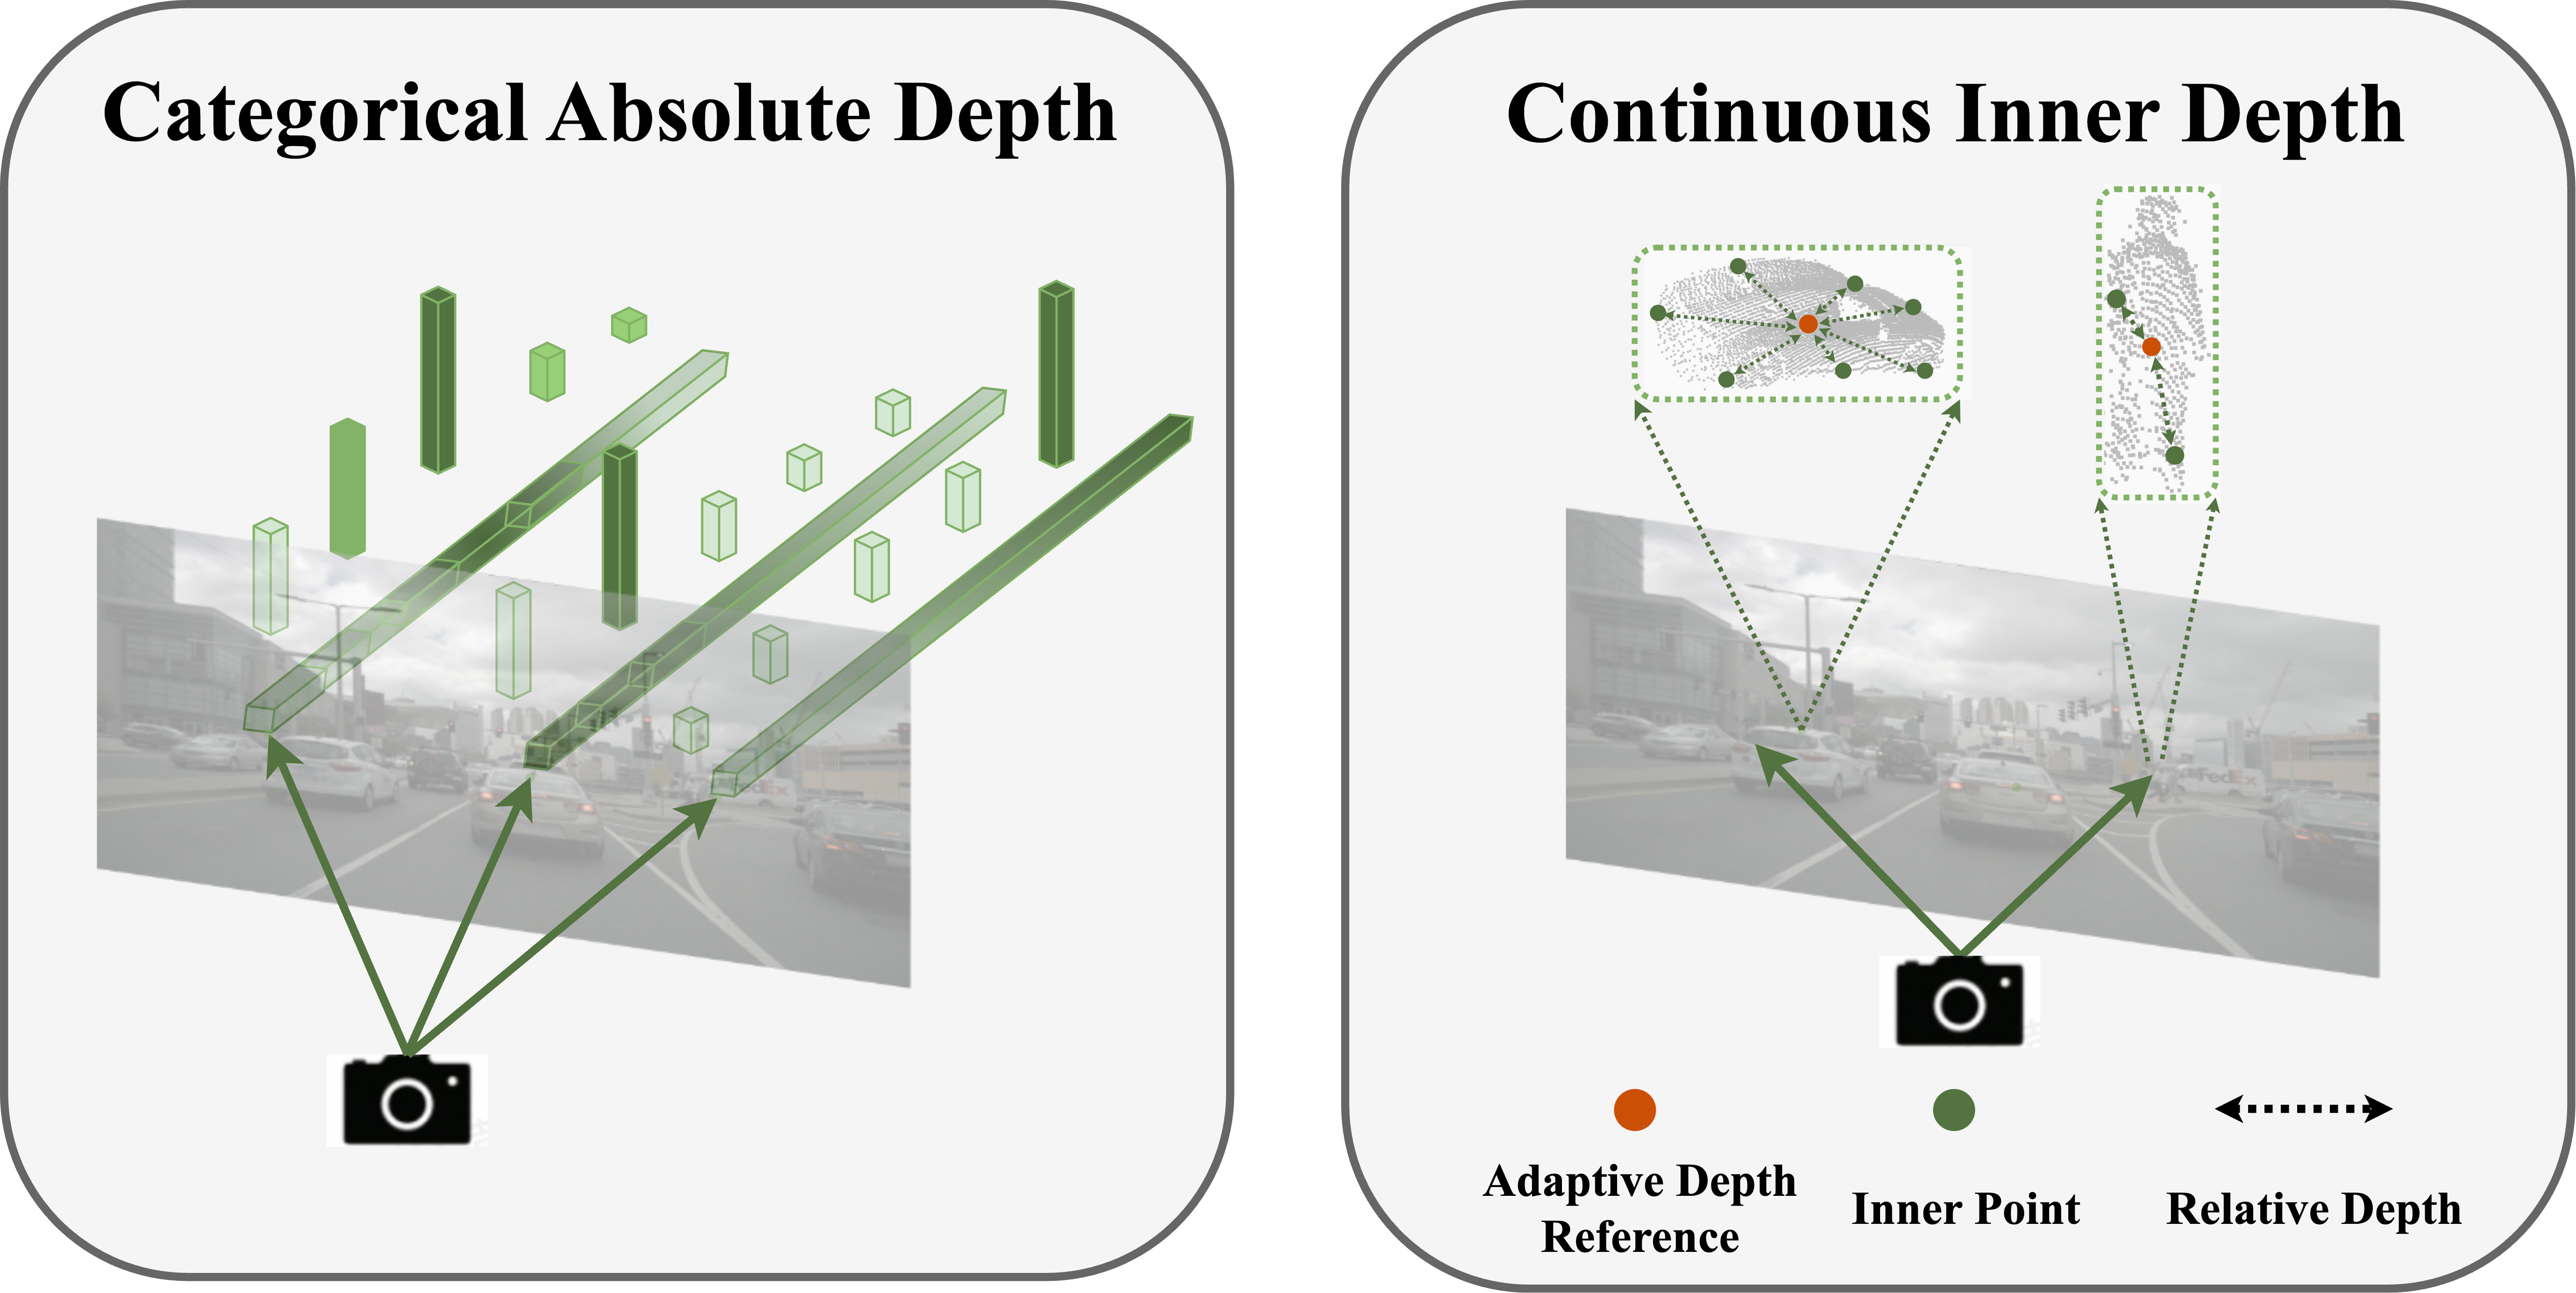
\includegraphics[scale=0.042]{cvpr_2022/iccv_fig5.drawio.png}
    \caption{\textbf{Comparison of Categorical Absolute Depth and Continuous Inner Depth.} We adopt the inner-depth supervision with continuous depth values to guide the camera-based student to learn local spatial structures of foreground object targets.
    }
    \label{fig:relative_depth}
    % \vspace{-0.8cm}
\end{figure}

%Start with $N$ ground truth 3D bounding boxes $\bm{B_{gt}}= \{\bm{b}_{i}\}_{i=1}^{N}$, which contains box center position, size and heading angle. We then obtain points in each 3D bounding boxes $\bm{P_{gt}}= \{\bm{P}^{pc}_i\}_{i=1}^{N}$, ${P}^{pc}_i$ means point clouds $P$ within 3d bounding box ${b}_{i}$. Take an object instance as example, we project ${P}^{pc}_i$ on image coordinate. 

%\begin{equation}
%    \hat{P_i^{}}(ud, vd, d) = K_{i}(R_i P_{i} + t_i),
%\end{equation}
 %In the section 3.1, we consider the depth estimation as a classification problem of the depth distribution. For the defined depth bins $b_i$, we interpret the $D$ Softmax scores, $p_k$, $k=1,..,D$, and choose the final prediction depth $b^{k}_i$ at highest prediction confidence bin. 

% In the absolute depth supervision, we apply one hot encoding to ${D_i}^{gt}$ considering the depth estimation as a classification problem of the depth distribution, first adopted in BEVDepth \cite{b7}. We divided the depth distance into D depth bins, the depth-bin-centers set denoted as ${\mathbf{B_i}=\{b^1_i, b^2_i,..., b^k_i,... b^D_i\}}$ , and we interpret the $D$ Softmax scores, $p^{k}_i$, $k=1,..,D$ at each pixel as probabilities over the ${\mathbf{B_i}}$ vector, and choose the final prediction depth $b^{k}_i$ at highest prediction confidence bin. 
%  \begin{equation}
%  \label{eq:FM}
%  \begin{aligned}
%     D_i = b^{k}_i {\max_{k=1}^D {{p^{k}_i}}}.
%  \end{aligned}
%  \end{equation}
% Here, we want to calculate the exact relative depth for different pixels within the target, the discrete depth prediction like above is not enough to express the tiny depth difference. Thus, for the further accurate prediction depth and can be used for the relative depth relation among different pixels within the certain ROI, we calculate the final depth value $\hat{D_i}$ by the hybrid mean regression as follow:
%  \begin{equation}
%  \label{eq:FM}
%  \begin{aligned}
%     {\hat{D_i}} = {\sum_{k=1}^D {{b^{k}_i}{p^{k}_i}}}.
%  \end{aligned}
%  \end{equation}
 % Compared the discrete depth prediction, we do not predict the depth as the chosen likely bin. This enables us to predict smooth depth without the discriminative artifacts, which helps to obtain the complete representation of the geometry depth.  
 
 \paragraph{Adaptive Depth Reference.}
 To calculate the relative depth values, we propose to utilize an adaptive depth reference for different foreground targets.
 Specifically, according to the predicted continuous depth values in $\{\hat{S_j}\}_{j=1}^M$, we select the pixel with the smallest depth prediction error as the reference point for each target, and correspondingly set its depth value as the depth reference, as shown in Figure~\ref{fig:relative_depth}. For the $j$-th target with the ground-truth inner-depth $\{\hat{S_j}, \hat{S^{gt}_j}\}_{j=1}^M$, we calculate the depth reference point $(x_r, y_r)$ by
  \begin{equation}
 \label{eq:FM}
 \begin{aligned}
    (x_r, y_r) = \mathop{\text{Argmin}}_{(x, y)\in \hat{S_j}} \left ({S^{gt}_j}(x, y) - {\hat{S_j}}(x, y)\right ).
 \end{aligned}
 \end{equation}
 Then, the predicted and ground-truth reference depth values are denoted as $d_j(x_r, y_r)$ and $d^{gt}_j(x_r, y_r)$, respectively. By adaptively selecting the reference point with the smallest error, the inner-depth distribution can dynamically adapt to objects with different shapes and appearances, which stabilizes the network learning for some truncated and occluded objects.

\paragraph{Inner-depth Calculation.}
On top of the reference depth value, we calculate the relative depth values within the foreground area of each target object. For pixel $(x, y)$ of the $j$-th target $\{\hat{S_j}, S_j^{gt}\}$, the predicted and ground-truth inner-depth values are formulated as
\begin{equation}
 \label{eq:FM}
 \begin{aligned}
    rd_j(x, y) &= d_j(x, y) - d_j(x_r, y_r),\\
    rd^{gt}_j(x, y) &= d^{gt}_j(x, y) - d^{gt}_j(x_r, y_r).
 \end{aligned}
 \end{equation}
 We denote the obtained relative depth-value sets for $M$ target objects as $\{\hat{R_j}, R_j^{gt}\}_{j=1}^M$. Finally, we supervise the inner-depth prediction of the student detector by an L2 loss, formulated as
 \begin{equation}
\label{eq:FM}
    \mathcal{L}_{\rm{depth}}^{R} = \sum_{j=1}^M ||\hat{R}_{j}-R^{gt}_{j}||_2.
\end{equation}
 
%  When we set the inner point and the reference point within the ROI, we can define the two relative depth sets ${\mathbf{\hat{D}}^{gt}}$ ${\mathbf{\hat{D}}^{pred}}$ of the pixels with cardinality ${M}$. 
% \begin{equation}
%     {\mathbf{\hat{D}}^{gt}} = 
% \left[{\hat{D}^{gt}_{1r},\hat{D}^{gt}_{2r},\cdots,\hat{D}^{gt}_{ir},\hat{D}^{gt}_{Mr}}\right].
% \end{equation}
% \begin{equation}
%     {\mathbf{\hat{D}}^{pred}} = 
% \left[{\hat{D}^{pred}_{1r},\hat{D}^{pred}_{2r},\cdots,\hat{D}^{pred}_{ir},\hat{D}^{pred}_{Mr}}\right].
% \end{equation}
%  where the ${\hat{D}_{ir}^{gt}}=\hat{D}_i^{gt}-\hat{D}_r^{gt}$ and ${\hat{D}_{ir}^{pred}=\hat{D}_i^{pred}-\hat{D}_r^{pred}}$ denotes the relative depth distance of the lidar pixels and cam pixels. 
 
%  To obtain the inner-geomtry depth relation from the lidar points, we minimize the discrepancy between the above sets in a one-to-one relative spatial matching manner. 
% \begin{equation}
% \label{eq:FM}
%     \mathcal{L}_{\rm{Rdepth}} = ||{\mathbf{\hat{D}}^{gt}}-{\mathbf{\hat{D}}^{pred}}||_2 = \sum_{i=1}^M ||\hat{D}^{gt}_{ir}-\hat{D}^{pred}_{ir}||_2.
% \end{equation}
%% \KY{focus on semantic mismatch}
%\noindent This formulation assumes that the semantic distributions of the teacher and the student match exactly. 
% However, a recent study~\cite{Cho2019OnTE} observes that small students are inefficient to mimic large teachers. 
%However, as mentioned earlier, for the feature maps of the teacher network, which usually encompasses more layers and larger feature channels, the spatial information of the same pixel location contains a richer semantic information compare to the student network. Directly regressing the features in a pixel-wise manner may lead to suboptimal distillation results. 
% has a stronger learning capability (\eg larger receptive field) and richer representation. That means the semantic of spatial components of teacher and student usually varies. Directly linking the teacher and student by spatial order may trigger the issues of semantic mismatch and lead to sub-optimal results.
% \KY{this is not helping the story, size difference is one reason that KD is hard. but our approach does not help in this way} 
% As the teacher grows in capacity and accuracy, the student often finds it difficult to emulate the teacher. 
% To this end, we propose to guide the whole student to mimic each spatial component of the teacher respectively. In this way, we can increase the matching capability and subsequently improve the knowledge distillation performance.

%This formulation does not consider the gap of expressivity and the exact semantic distance between $f^s_i$ and $f^t_i$, which may introduce bias. To address the limitation of Eq. \ref{eq:FM}, we reconfigure each elements in set $f^s$ by a target-aware transformer. 
%A straightforward solution is to measure the semantic distance between the elements of two sets and then assign the $f^t_i$ with the most semantic-related one from $f^s$. As we will demonstrate, this is the special case of our proposed method.
%To this end, we propose a one-to-all spatial matching knowledge distillation pipeline that allows the each feature location of the teacher to teach the entire student features in a dynamic manner.
%To make the whole student mimic a spatial component of the teacher, we propose the \textbf{T}arget-\textbf{a}ware \textbf{T}ransformer (\textbf{TaT}) to pixel-wisely reconfigure the semantic of student feature in the certain position.
%We propose the Target-aware Transformer (\textbf{TaT}) to pixel-wisely reconfigure the semantic of student feature in the certain position. 
%Given a spatial component (alignment target) of the teacher, we use \textbf{TaT} to guide the whole student to reconstruct the feature in its corresponding location. Conditioned on the alignment target,  \textbf{TaT} should reflect the semantic similarity with the components of the student feature. We use a linear operator to avoid changing the distribution of student semantics. The formulation of transformation operator $W^i$ can be defined as:
%Given the alignment target $f^t_i$, \textbf{TaT} is to find the weights $W^i$ that controls the flow of semantic aggregation across the student feature w.r.t the $i$-th pixel of student feature. Conditioned on the alignment target, \textbf{TaT} should reflect the semantic similarity with the components of the student feature. Also, it should be a linear operator otherwise it changes the distribution of student semantics. The formulation of $W^i$ can be defined as:
%\begin{equation}
%\label{eq:spe}
%\begin{aligned}
%   W^i&= \sigma(\langle {f^s_1},{f^t_i}\rangle,\langle {f^s_2},{f^t_i}\rangle,\dots,\langle {f^s_N},{f^t_i}\rangle)\\
%   &=[{w^i_1},{w^i_2},\dots,{w^i_N}],
%\end{aligned}
%\end{equation}
%\noindent where $f^t_i$ and $f^s_i$ denote the corresponding $i$-th components of teacher and student, $\langle \cdot,\cdot \rangle$ represents the inner-product and  $\|W^{i}\|=1$. We use inner-product to measure the semantic distance and softmax function for normalization. 
%Note that if we only reserve the entry of the maximum of $W^{'}$, it degrades to the nearest-neighbor. 
% Here $W^{i}$ is the gate that guides the semantic flow to the reconfigured point ${f^s_i}^{'}$. 



%Note this is the simple non-parametric method that only depends on the original features. To facilitate the training, we introduce the parametric method with the extra linear transformation applied on the student feature and teacher feature. We observe that parametric version performs better than non-parametric one in ablation study. Guided by the target-aware transformer, the reconfigured student feature can be formulated as: 
% \KY{why we need parameteric formulation? does non-param work? do we have the experiment? if not, consider to do this in supplementary}
% Also, the issue of semantic mismatching may occur in the channel dimension. To address this issue, we propose to partition the feature tensor along the channel dimension and performs the self-assembling in parallel:
%\begin{equation}
%\label{eq:mul-self-essem}
%    {f^s}^{'}=\sigma(\gamma(f^{s})\cdot \theta({f^t})^{\top})\cdot \phi(f^{s}),
%\end{equation}
%\noindent where $\theta(\cdot)$, $\gamma(\cdot)$ and $\phi(\cdot)$ are the linear functions consisting of $3\times 3$ conv layer plus the BN layer \cite{ioffe2015batch}. We compare the parametric \textbf{TaT} to non-parametric one to analyse the effectiveness brought by these linear functions in the Section~\ref{sec:ablation}. 
%In the case that the channel numbers of $F^S$ do not match with that of $F^T$, $\gamma(\cdot)$ can help with alignment.

% \KY{where? point the section} 
%The resulting \textbf{TaT} map ($\gamma(f^{s})\cdot \theta({f^t})^{\top}$) is of size $\mathbb{R}^{HW \times HW}$, which is acceptable considering that most classification networks have small feature map size on the top layers. On ResNet18, the spatial size of feature map in the 4-th block is, for example, $7\times7$.  \KY{discuss the complexity in the next section...}

%After reconfiguration, each component of ${f^s}^{'}$ aggregates the meaningful semantic from the original feature, which enhances the expressivity. We do not require the student to reconstruct the teacher feature in a pixel-to-pixel manner. Indeed, our model allows the student to act as a whole to mimic the teacher. The resulting ${f^s}^{'}$ is lately asked to minimize the L$_2$ loss with the teacher feature. The objective for \textbf{TaT} knowledge distillation can be given by:
%\begin{equation}
%    \mathcal{L}_{\rm{TaT}}= ||{f^s}^{'}-f^t||_2.
%    \label{eq:fm}
%\end{equation}

% \KY{this only apply to Cls? how about other loss? consider change cls $\rightarrow$ task. L_T -> $L_{TaT}$ }
%Finally, the total loss of our proposed method can be defined by: 

%\begin{equation}
%\label{eq:objective}
    %\mathcal{L}=\alpha\mathcal{L}_{\rm{Task}}+\beta\mathcal{L}_{\rm{KL}}+\epsilon\mathcal{L}_{\rm{TaT}},
%\end{equation}
%\noindent Here $\mathcal{L}_{\rm{Task}}$ can be any loss on the generic machine learning tasks. $\alpha$, $\beta$ and $\epsilon$ are the weight factors to balance the loss. 
%Empirically, we find that our model benefits from $\mathcal{L}_{\rm{KL}}$. However, the model can achieve state-of-the-art without the help of $\mathcal{L}_{\rm{KL}}$.
% , \ie, $\beta$ is set to 0. \KY{this is strange... why mentioning this if we set beta = 0??}

% \subsection{Empirical \& Theoretical Analysis}
% This section provides some intuition to the formulation discussed above. Without loss of generality, let's remove the linear functions $\theta(\cdot)$ and $\gamma(\cdot)$ and consider only one attention head. The Eq. \ref{eq:fm} can be expressed in another way:
% \begin{equation}
%     softmax(X\cdot Y^{\top})\cdot X=Y.
% \end{equation}
% \noindent Here $softmax(X\cdot Y)$ is the cross-attention matrix which is applied to the student feature $X$. The objective for the student is to reconstruct the teahcer feature. Denote the optimum solution to $X$ as $\hat{X}$. The non-trivial solution indeed requires that $softmax(\hat{X}\cdot Y^{\top})=I$ and $\hat{X}=Y$.

% Recall that each raw of $X$ and $Y$ corresponds to a pixel in the original feature tensor. By means of matrix multiplication, it calculates the inner-product of each paired pixels between student and teacher, resulting the cross-attention matrix. The inner-product between two pixels measures the similarity against difference, and it's normalized by the softmax function. Since the cross-attention matrix is required to be the identity matrix, this can be interpreted that the distance, reflected by the inner-product, of the associated positions between $f_s$ and $f_t$ should be as close as possible, otherwise distant. This is the necessary condition if $\hat{X}=Y$ holds.

% We now begin to give a theoretical analyse to the existence of the solution $\hat{X}$. Because student feature is expected to match the teacher feature, we have $\hat{X}=Y$. Thus, we need to prove that $softmax(Y,Y^{\top})=I$. We presume that the elements of $Y$ is Gaussian distribution and each raw is not linearly dependent from each other. Here $Y$ can be represented as:
% \begin{equation}
% \begin{aligned}
%   Y=[{y_1}^{\top},{y_2}^{\top},{y_3}^{\top},\dots,{y_N}^{\top}]^{\top},\\
% \end{aligned}
% \end{equation}
% \noindent where $Y$ has $N=H\cdot W$ raw vectors. Suppose that $y_i$ and $y_j$ are two distinct vectors, they can be described as:
% \begin{equation}
% \begin{aligned}
%   y_i=[y_{i,1},y_{i,2},y_{i,3},\dots,y_{i,C}],\\
%   y_j=[y_{j,1},y_{j,2},y_{j,3},\dots,y_{j,C}],\\
% \end{aligned}
% \end{equation}
% where $(1\leq i,j\leq N)$ and each vector is of length $C$. The expected value of the inner-product of two vectors can be given by:
% \begin{equation}
% \label{eq:in_prd_same}
%     \begin{aligned}
%       \mathbb{E}\langle y_i,y_i\rangle &= \mathbb{E}(y_{i,1}^2+y_{i,2}^2+y_{i,3}^2+\dots+y_{i,C}^2) \\
%       &=\sum_{k=1}^{C}\mathbb{E}y_{i,k}^2= \sum_{k=1}^{C}(\mu_{i,k}^2+\sigma_{i,k}^2)=C ,
%     \end{aligned}
% \end{equation}

% \begin{equation}
% \label{eq:in_prd_diff}
%     \begin{aligned}
%       \mathbb{E}\langle y_i,y_j\rangle 
%       &= \mathbb{E}(y_{i,1}\cdot y_{j,1}+y_{i,2}\cdot y_{j,2}+\dots+y_{i,C}\cdot y_{j,C}) \\
%       &=\sum_{k=1}^{C}\mathbb{E}(y_{i,k}\cdot y_{j,k})\\
%       &=\sum_{k=1}^C \left[ \mathbb{E}y_{i,k}\cdot \mathbb{E}y_{j,k}+Cov(y_{i,k},y_{j,k}) \right]  \\
%       &\leq \sum_{k=1}^{C}(\mu_{i,k}\cdot \mu_{j,k}+|\sigma_{i,k}\cdot \sigma_{j,k}|)\\
%       &=\rho \cdot C .
%     \end{aligned}
% \end{equation}
% Here $\mu=0$ and $\sigma=1$ is the mean and standard deviation of Gaussian distribution. The Eq. \ref{eq:in_prd_same} indicates the expected value of the inner-product between a vector and itself, while Eq. \ref{eq:in_prd_diff} illustrates the inner-product of two distinct vectors, which is derived by Cauchy–Schwarz inequality a.k.a covariance inequality. Here $0\leq \rho \leq 1$ and it equals to 1 if and only if two vectors are linearly dependent. Since we presume that vectors are not linearly dependent in matrix $Y$, we have $\rho<1$.

% Given Eq. \ref{eq:in_prd_same} and Eq. \ref{eq:in_prd_diff}, we consider the diagonal of the cross-attention matrix. Normalized with softmax function, the limiting condition of the $i$-th position of the $i$-th raw can be described by:
% \begin{equation}
% \label{eq:lim}
%     \lim_{C\to \infty} \frac{e^C}{(N-1)\cdot e^{\rho\cdot C}+e^C}=1.
% \end{equation}

% The limiting condition presented in Eq. \ref{eq:lim} means the $i$-th raw of the cross-attention map is the one-hot vector where $i$-th position is 1 as long as the feature channel is deep enough. Thus the resulting cross-attention matrix is an identity matrix. In our experiment setting, the feature tensor of 4-th layer in ResNet18 is of size $7\times 7 \times 512$, \ie $N=49$ and $C=512$. Even though $\rho$ reaches 0.98, Eq. \ref{eq:lim} can return 0.998 that is very close to 1.  

%--------------------------------------------------------------------------------

%--------------------------------------------------------------------------------
\subsection{Inner-feature BEV Distillation}
\label{sec:Inner-feature BEV Distillation}
%In this section we introduce the adaption of the model discussed previously and show its application on semantic segmentation. 
% \KY{inductive bias? do we really want to talk about this?}
% \ky{Although our one-to-all distillation approach can address the semantic mismatch, it has one limitation about the computational complexity. As the resulting correlation mapping }
% The proposed \textbf{TaT} lift the limitation of previous one-to-one spatial matching fashion. 
%For example, features in the neighborhood are more relevant to themselves, on the contrary, features that are farther away are less relevant. The student must figure out all of these in the learning process, which may be very challenging when the feature map is large.

Besides the depth supervision for low-level spatial information, our TiG-BEV also adopts the inner-geometry learning for high-level BEV semantics from pre-trained LiDAR-based detectors. 
Previous works~\cite{b9,b52} for BEV distillation directly force the student to imitate the teacher's features point-to-point in the BEV space. In spite of the performance improvement, such strategies are constrained by the following two aspects. On the one hand, due to the sparsity of scanned point clouds, the LiDAR-based BEV features might contain redundant and noisy information in the background areas. Although BEVDistill~\cite{b9} utilizes foreground masks to alleviate this issue, such dense feature distillation still cannot provide focused and effective guidance to the student network. On the other hand, the camera-based and LiDAR-based BEV features depict different characteristics of the scene, respectively, visual appearances and spatial structures. Therefore, forcing the BEV features to be completely consistent between two modalities is sub-optimal considering the semantic gap. In our TiG-BEV, we propose an inner-feature BEV distillation (Figure~\ref{fig:structure_attn}) consisting of inter-channel and inter-keypoint learning schemes, which conducts attentive target features distillation and relieve the cross-modal semantic gap.

% There are two main observations, on the one hand, the feature distribution of point clouds and images are not consistent due to the sparsity of point clouds, directly distilling on all region of features is not reasonable. On the other hand, even features of two modalities can hold meaningful information in the region of foreground, the representation of the features from different modalities are diverse in channel and spatial wise. Forcing students to imitate the foreground feature of the teacher is sub-optimal. Therefore, we propose a foreground structured attention feature supervision module to transfer more reliable relative spatial feature relationships from LiDAR-based teacher to multi-view based student. It contains of two distillation modules: 1) Inner Target-Aware distillation, 2) Local Target-Aware distillation,which..


\paragraph{Target Keypoint Extraction.}
To distill the knowledge of LiDAR-based detectors only within sparse foreground regions, we extract the BEV area of each object target and represent it by a series of keypoint features.
Given the ground-truth 3D bounding box for each target, we first enlarge the box size for a little bit in the BEV space to cover the entire foreground area, e.g., object contours and edges. Then, we uniformly sample its BEV bounding box by $N$ keypoints, and adopt bilinear interpolation to obtain the keypoint features from the encoded BEV representations. From both camera-based $F^{2d}_{\rm bev}$ and LiDAR-based $F^{3d}_{\rm bev}$, we respectively extract the keypoint features for all $M$ object targets as $\{f_j^{2d}, f_j^{3d}\}_{j=1}^M$, where $f_j^{2d}, f_j^{3d} \in {\mathbb{R}^{N\times C}}$. By the uniform sampling, such BEV keypoints can well represent the part-wise features and the inner-geometry semantics of foreground targets.

\begin{figure}[!t]
% \vspace{-0.5cm}
    \centering
    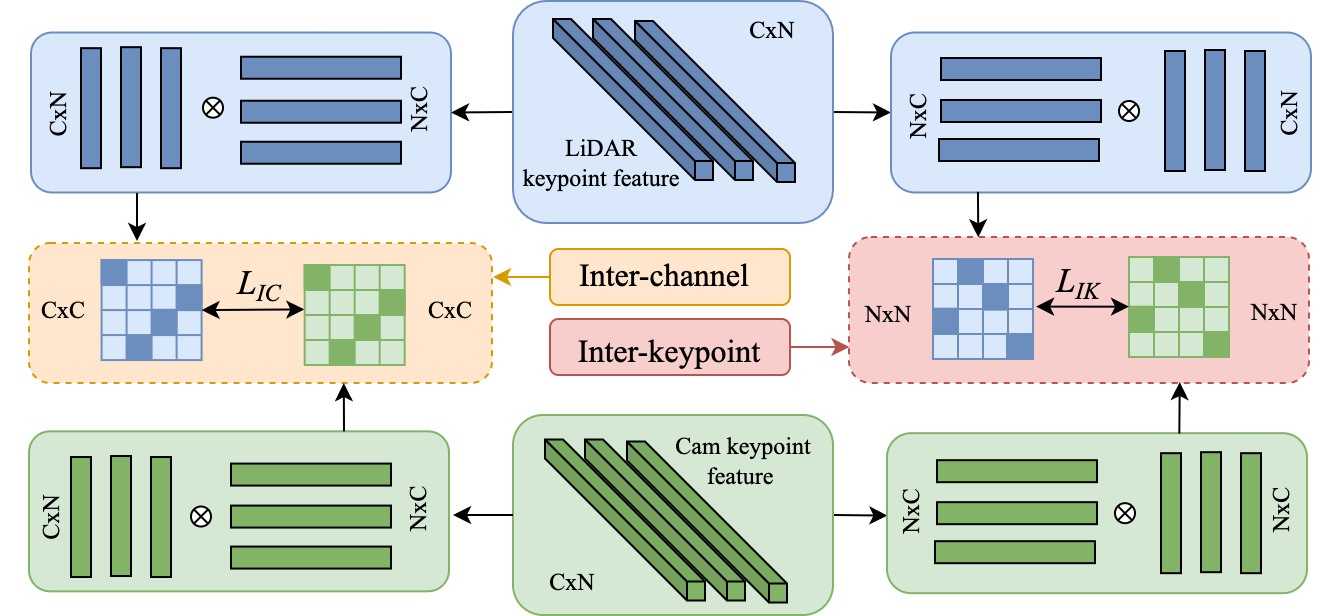
\includegraphics[scale=0.17]{cvpr_2022/iccv_fig6_2.drawio.png}
    \caption{\textbf{Detials of Innter-feature BEV Distillation.} For each foreground area in BEV space, we represent rach target feature by a set of keypoints and conduct feature distillation in both inter-channel and inter-keypoint manners.
    }
    \label{fig:structure_attn}
    % \vspace{-0.8cm}
\end{figure}

% and the corresponding background regions and divide into small grids with spatial resolution of $G_i\times G_i \times G_i$, which can summarize each foreground area into the certain number of feature keypoints.  For the bird-view feature maps, we project the keypoint $p_i$ to the 2D bird-view coordinate system and utilize bilinear interpolation to obtain the features $f^{bev}_i$ from the bird-view feature maps. Hence, the roi feature can be represented as follow:

% \begin{equation}
%     {F_i^{ROI}} = {f^{bev}_1,...,f^{bev}_i,f^{bev}_n}, 
%  i=1,..N
% \end{equation}
% which have the strong capability of preserving 3D geometry information of the foreground scene and can also boost the marginal awareness performance of the certain target.

\paragraph{Inter-channel BEV Distillation.}
% \label{sec:seq}
Taking the $j$-th object target as an example, we first apply an inter-channel BEV distillation, which guides the student keypoint features to mimic the channel-wise relationships of the teacher's. Such inter-channel signals imply the overall geometric semantics of each object target. Compared with the previous channel-by-channel supervision, our inter-channel distillation can preserve the distinctive aspects of the two modalities, while effectively transfer the well pre-trained knowledge of LiDAR-based detectors. Specifically, we calculate the inter-channel similarities of both camera-based and LiDAR-based keypoint features, formulated as
\begin{equation}
    A_j^{2d} = f_j^{2d} {f_j^{2d}}^{\top};\ \ \ A_j^{3d} = f_j^{3d} {f_j^{3d}}^{\top},
\end{equation}
where $A_j^{2d}, A_j^{3d} \in {\mathbb{R}^{C\times C}}$ denote the feature relationships between different $C$ channels for the two modalities. For all $M$ objects in a scene, we adopt L2 loss between the two inter-channel similarities for feature distillation, formulated as
\begin{equation}
    \mathcal{L}_{\rm{bev}}^{{IC}}= \sum_{j=1}^{M} ||A_j^{3d}-A_j^{2d}||_2.
    \label{eq:fm}
\end{equation}

% Given the RoI feature of each box proposal, the lidar-based bev feature and cam-based bev feature can be represented as $F_i^{Lidar}\in {\mathbb{R}^{N\times C}}$, $F_i^{cam}\in {\mathbb{R}^{N\times C}}$ respectively, where ${N}$ represents the number of keypoints and ${C}$ represents the channels numbers. For the certain sampled feature of the keypoint, it reflects the certain information within the receptive field. As mentioned before, the lidar-based detector has the better detection performance since the spatial information of the same inner roi location contains the richer semantic information compare to the cam-based detector. Thus, we propose a inner target-aware (\textbf{ITA}) distillation that performs distillation within channel wise, which allows student to learn the context of feature from RoI patches and retain the correlation among different channels. For the bev feature ${i}$th ROI, the channel-wise information matrix is defined as: 
% \begin{equation}
%     {G_i^{ROI}} = {F^{Lidar}_i\cdot {F^{Lidar}_i}}^{\top}
% \end{equation}
% The information matrix has a size of ${C\times C}$ regardless of the spatial dimension ${N}$. ${G_{i,(m,n)}^{ROI}}$ denotes the inner channel correlation between $m$th channel and $n$th channel for the same location of the $i$th ROI.

% \begin{equation}
% \begin{aligned}
% %L_{task} = &\lambda_1 L_{per}(G_s(x),G_t(x))  +\lambda_1  L_{CE}(y,\delta(z_s))\\ & + \lambda_1L_{Focal}(y,y_{out})
% %{G_{i,(m,n)}^{ROI}} = &{f^_{1,m}}{f^_{1,n}}^{\top}  +{f^_{2,m}}{f^_{2,n}}^{\top} + \dots + \\&{f^_{N,m}}\cdot {f^_{N,n}}^{\top}
% {G_{i,(m,n)}^{ROI}} = &{f^_{1,m}}\cdot {f^_{1,n}}^{\top} + {f^_{2,m}}\cdot {f^_{2,n}}^{\top}\\ & + \dots + \\{f^_{N,m}}\cdot {f^_{N,n}}^{\top}
% \end{aligned}
% \end{equation}


% For the same roi area, to make the whole cam-based detector mimic
% a spatial component of the lidar-based detector, we use the Inner-target aware operator ${G_{i,(m,n)}^{ROI}}$ to pixel-wisely reconfigure the
% semantic of cam-based feature in the certain position and transfer the channel correlation of the lidar-based feature to the cam-based feature in the certain position. Conditioned on the same roi, the ${G_{i,(m,n)}^{ROI}}$ should reflect the semantic similarity with between the components. 

% We penalize the $L_2$ distance between the channel-wise information matrix of the lidar-based detector and the cam-based detector, allowing the cam-based to obtain the similar feature diversity for the same foreground area.
% \begin{equation}
%     \mathcal{L}_{\rm{ITA}}= ||G^{Lidar}_{i,cha}-G^{cam}_{i,cha}||_2.
%     \label{eq:fm}
% \end{equation}


\begin{table*}[ht]
\centering
\caption{\textbf{Performance Comparison on nuScenes~\cite{b6} Val Set.} 'C' and 'L' denote the camera-based and LiDAR-based methods, which refer to the input data during inference. * denotes our implementation using BEVDet\cite{b19} codebase.
%using their official codes.
% We have at least 1 absolute point of performance gain against KD \cite{Hinton2015DistillingTK} on 5 out of 7 experimental settings.
}
%\vspace{-0.2cm}
\resizebox{2\columnwidth}{!}{
\tablestyle{5pt}{1.2}
\begin{tabular}{c|c|c|c|cc|ccccc}
\toprule[1.2pt]
Method          & Modality & Backbone & Resolution & mAP↑  &NDS↑& mATE↓ & mASE↓ & mAOE↓ & mAVE↓ & mAAE↓   \\ \midrule
FCOS3D\cite{b12}          & C  &ResNet-101 & 900 $\times$ 1600 & 0.343& 0.415 & 0.725 & 0.263 & 0.422 & 1.292 & 0.153  \\
PGD\cite{b17}             & C  &ResNet-101 & 900 $\times$ 1600 & 0.369& 0.428 & 0.683 & 0.260 & 0.439 & 1.268 & 0.185  \\
MonoDETR\cite{b47}             & C  &ResNet-101 & 900 $\times$ 1600 & 0.372& 0.434 & 0.676 & 0.258 & 0.429 & 1.253 & 0.176  \\
%BEVDepth-R50        & C &ResNet-50   & 256 \times 704  & 0.351 & 0.639 & 0.267 & 0.479 & 0.428 & 0.198 & 0.475 \\
% BEVDepth\cite{b7}         & C &ResNet-101  & 512 \times 1408 & 0.412 & 0.565 & 0.266 & 0.358 & 0.331 & 0.190 & 0.535 \\
DETR3D\cite{b13}          & C &ResNet-101  & 900 $\times$ 1600 & 0.303& 0.374 & 0.860 & 0.278 & 0.437 & 0.967 & 0.235  \\
PETR\cite{b21}            & C  &ResNet-101    & 512 $\times$ 1408 & 0.357 & 0.421& 0.710 & 0.270 & 0.490 & 0.885 & 0.224  \\
BEVFormer\cite{b11}       & C  &ResNet-101   & 900 $\times$ 1600 & 0.416 & 0.517& 0.673 & 0.274 & 0.372 & 0.394 & 0.198   \\
PETRv2\cite{b24}            & C  &ResNet-101    & 640 $\times$ 1600 & 0.421& 0.524 & 0.681 & 0.267 & 0.357 & 0.377 & 0.186  \\
MonoDETR-MV\cite{b48}            & C  &ResNet-101    & 640 $\times$ 1600 & 0.428 & 0.531 & 0.676 & 0.268 & 0.352 & 0.380 & 0.169  \\ \midrule
CenterPoint~\cite{b53} (Teacher)   & L &VoxelNet   & -          & 0.564 & 0.646& 0.299 & 0.254 & 0.330 & 0.286 & 0.191  \\ \midrule
BEVDet$^*$ \cite{b19} & C &ResNet-50   & 256 $\times$ 704 & 0.298& 0.379 & 0.725 & 0.279 & 0.589 & 0.860 & 0.245  \\ 
\rowcolor{gray!12} \textbf{+ TiG-BEV}     &C  &ResNet-50  & 256 $\times$ 704 & \textbf{0.331} & \textbf{0.411}& 0.678 & 0.271 & 0.589 & 0.784 & 0.218  \\ 
\rowcolor{gray!12}& &&& \textbf{\textcolor{blue}{+3.3$\%$} }& \textbf{\textcolor{blue}{+3.2$\%$}}&\textcolor{blue}{-4.7$\%$} & \textcolor{blue}{-0.8$\%$} & \textcolor{blue}{-0.0$\%$} & \textcolor{blue}{-7.6$\%$} & \textcolor{blue}{-2.7$\%$}   \\ 
\midrule
BEVDet4D$^*$ \cite{b23} & C &ResNet-50   & 256 $\times$ 704 & 0.322 & 0.451& 0.724& 0.277& 0.520 &0.366 &0.212  \\
\rowcolor{gray!12} \textbf{+ TiG-BEV}     & C &ResNet-50  & 256 $\times$ 704 & \textbf{0.356}& \textbf{0.477} & 0.648 & 0.273 & 0.517 & 0.364 & 0.210  \\ 
\rowcolor{gray!12}& &&& \textbf{\textcolor{blue}{+3.4$\%$} }& \textbf{\textcolor{blue}{+2.6$\%$}}&\textcolor{blue}{-7.6$\%$} & \textcolor{blue}{-0.4$\%$} & \textcolor{blue}{-0.3$\%$} & \textcolor{blue}{-0.2$\%$} & \textcolor{blue}{-0.2$\%$}   \\ 
\midrule
BEVDepth$^*$ \cite{b7} & C &ResNet-101   & 512 $\times$ 1408 & 0.416 & 0.521& 0.605 & 0.268 & 0.455 & 0.333 & 0.203  \\
\rowcolor{gray!12}   \textbf{+ TiG-BEV}   & C & ResNet-101  & 512 $\times$ 1408  & \textbf{0.440}& \textbf{0.544} & 0.570 & 0.267 & 0.392 & 0.331 & 0.201  \\ 
\rowcolor{gray!12}& &&& \textbf{\textcolor{blue}{+2.4$\%$} }& \textbf{\textcolor{blue}{+2.3$\%$}}&\textcolor{blue}{-3.5$\%$} & \textcolor{blue}{-0.1$\%$} & \textcolor{blue}{-6.3$\%$} & \textcolor{blue}{-0.2$\%$} & \textcolor{blue}{-0.2$\%$}   \\ 
\bottomrule[1.2pt]
\end{tabular}
}

\label{tab:nus_val_sota}
%\vspace{-3mm}
\end{table*}
\paragraph{Inter-keypoint BEV Distillation.}
\label{sec:anchor}
The inter-channel distillation guides the camera-based detector to learn the channel-wise diversity from the LiDAR-based teacher. However, it is conducted without considering the inner correlation of different keypoints within each object target, which is not capable of capturing the local geometries among different foreground parts, e.g., the front and rear of cars. To this end, we propose to utilize the inter-keypoint correlations of LiDAR-based BEV features and transfer such inner-geometry semantics into camera-based detectors. Analogous to the aforementioned inter-channel module, for the $j$-th target object, we calculate the inter-keypoint similarities in a transposed manner for the two modalities as
\begin{equation}
    B_j^{2d} = {f_j^{2d}}^{\top} {f_j^{2d}};\ \ \ B_j^{3d} = {f_j^{3d}}^{\top} {f_j^{3d}},
\end{equation}
where $B_j^{2d}, B_j^{3d} \in {\mathbb{R}^{N\times N}}$ denote the feature relationships between different $N$ keypoints respectively for camera and LiDAR. We also adopt L2 loss for all $M$ targets as
\begin{equation}
    \mathcal{L}_{\rm{bev}}^{{IK}}= \sum_{j=1}^{M} ||B_j^{3d}-B_j^{2d}||_2.
    \label{eq:fm}
\end{equation}
Then, the distillation loss for inter-channel and inter-keypoint features in BEV space is formulated as
\begin{equation}
    \mathcal{L}_{\rm{bev}}=
    \mathcal{L}_{\rm{bev}}^{{IC}}+
    \mathcal{L}_{\rm{bev}}^{{IK}},
    \label{eq:seg}
\end{equation}
where the two terms are orthogonal respectively for the channel-wise feature diversity and keypoint-wise semantic correlations.

% The attempt to preserve the local correlation through concatenating all the position would fail. 
% We hope that detector can capture the context from the one position to another within the target area. In this case, the cam-based detector will, however, be distracted from the locality since the \textbf{ITA} encodes all the related semantic over the whole feature among different positions. In other words, the \textbf{ITA} will aggregates redundant local semantic.
% Furthermore, a large feature map will hinder the inductive bias since it may encourage the student to integrate the less relevant semantic from remote positions by mistake, which may deteriorate the subsequent distillation performance.
% For complex scenes and similar targets, the postion wise dependency is important to capture the relation (\eg layout) of different components within the target.

% We address the conundrum by the proposed local target-aware(\textbf{LTA}) distillation. Like the the channel-wise information matrix defined in \textbf{ITA}, the position-wise matrix is defined as follow:
% \begin{equation}
%     {G_{i}^{pos}} = {{F^{Lidar}_i}^{\top}\cdot F^{Lidar}_i}
% \end{equation}

% The information matrix has the size of ${N\times N}$ regardless of the channel dimension ${C}$. ${G_{i,(p,q)}^{pos}}$ denotes the inner spatial correlation between $p$th keypoint and $q$th keypoint for the $i$th ROI. Similarly, the formulation of the operator can be defined as:

% \begin{equation}
% \begin{aligned}
%     {G_{i,(p,q)}^{pos}} = {f^_{p,1}}\cdot {f^_{q,1}}^{\top} + {f^_{p,2}}\cdot {f^_{q,2}}^{\top} + \dots + \\{f^_{p,C}}\cdot {f^_{q,C}}^{\top}
% \end{aligned}
% \end{equation}

% After reconfiguration, the spatial relationship within the target can be extracted and summerized, which is complementary to the channel relationship. Therefore, as the cam-based detector, we enhance its gemetry expressivity by asking them to mimic the teacher. Thus, the objective for (\textbf{LTA}) knowledge distillation can be given by:

% \begin{equation}
%     \mathcal{L}_{\rm{LTA}}= ||G^{Lidar}_{i, pos}-G^{Cam}_{i, pos}||_2.
%     \label{eq:fm}
% \end{equation}

\subsection{Overall Loss}
\label{sec:overall_loss}
To sum up, we benefit the student camera-based detector by target inner-geometry from two complementary aspects, i.e., an inner-depth supervision for low-level signals and an inner-feature BEV distillation for high-level semantics. They produce two losses as $\mathcal{L}^R_{\rm{depth}}$ and $\mathcal{L}_{\rm{bev}}$. Together with the original two losses, i.e., dense absolute depth supervision $\mathcal{L}^A_{\rm{depth}}$, and 3D detection $\mathcal{L}_{\rm{det}}$, the overall loss of our TiG-BEV is formulated as
\begin{equation}
    \mathcal{L}_{\rm{TiG}}=
    \mathcal{L}_{\rm{det}}+
    \mathcal{L}^A_{\rm{depth}}+
    \mathcal{L}^R_{\rm{depth}}+
    \mathcal{L}^{IC}_{\rm{bev}}+
    \mathcal{L}^{IK}_{\rm{bev}}.
    \label{eq:seg}
\end{equation}

% The inner target-aware distillation enables the detector to mimic the inner feature diversity while the local target-aware distillation allows it to learn the local representation over the spatial feature, which are complementary to each other. Therefore, the combination of these two objectives can bring the best of two worlds. Our objective designed for structured attention feature supervision can be written by:
% \begin{equation}
%     \mathcal{L}_{\rm{SAF}}=
%     \delta\mathcal{L}_{\rm{ITA}}+
%     \zeta\mathcal{L}_{\rm{LTA}}
%     \label{eq:seg}
% \end{equation}



% Finally, the total loss of our proposed method can be defined by:
% \begin{equation}
%     \mathcal{L}_{\rm{TiG}}=
%     \mathcal{L}_{\rm{det}}+
%     \mathcal{L}^A_{\rm{depth}}+
%     \mathcal{L}^R_{\rm{depth}}+
%     \mathcal{L}^{IC}_{\rm{bev}}+
%     \mathcal{L}^{IK}_{\rm{bev}}
%     \label{eq:seg}
% \end{equation}
% Here $L_{task}$ is the loss of the 3D detection task. $\alpha$, $\beta$, $\gamma$, $\delta$ and $\zeta$ are the weight factors to balance the loss.


\section{Experiments}

\subsection{Communication Efficiency at Scale}\label{sect:experiments_square_cube}

Before we can meaningfully evaluate SWARM parallelism, we must verify our theoretical observations on communication efficiency. Here we run several controlled experiments that measure the GPU utilization and network usage for different model sizes, using the Transformer architecture~\citep{transformer} that has been widely adopted in various fields~\citep{lin2021survey}. To decouple the performance impact from other factors, we run these experiments on homogeneous V100 GPU nodes that serve one pipeline stage over the network with varying latency and bandwidth. We use a batch size of 1 and sequences of 512 tokens; the complete configuration is deferred to Appendix~\ref{appendix:detailed_setup}.


First, we measure how the model size affects the computation to communication ratio at 500 Mb/s network bandwidth in both directions. We consider 4 model configurations: the base configuration from the BERT paper~\citep{bert}, ``xxlarge" (``large'' with $d_{model}{=}4096$),  which is used in several recent works~\citep{albert,ernie3,deberta}, and a GPT-3-scale model with $d_{model}{=}12288$~\citep{gpt3}. We also evaluate a modified Transformer architecture (``Ours'') as defined in Section~\ref{sect:experiments_large} with $d_{model}{=}4096$, 3 layers per pipeline stage and 8-bit quantized activations. As we demonstrate in Appendix~\ref{appendix:compression}, this compression strategy can significantly reduce network usage with little effect on convergence. In the first three configurations, the model consists of 12 Transformer layers placed on 12 servers with a single GPU; in the last one, there are 4 servers, each hosting 3 layers.
Appendix~\ref{appendix:detailed_setup} contains FLOP and parameter counts of each configuration.




\begin{figure}[b]
\vspace{-14pt}
    \centering
    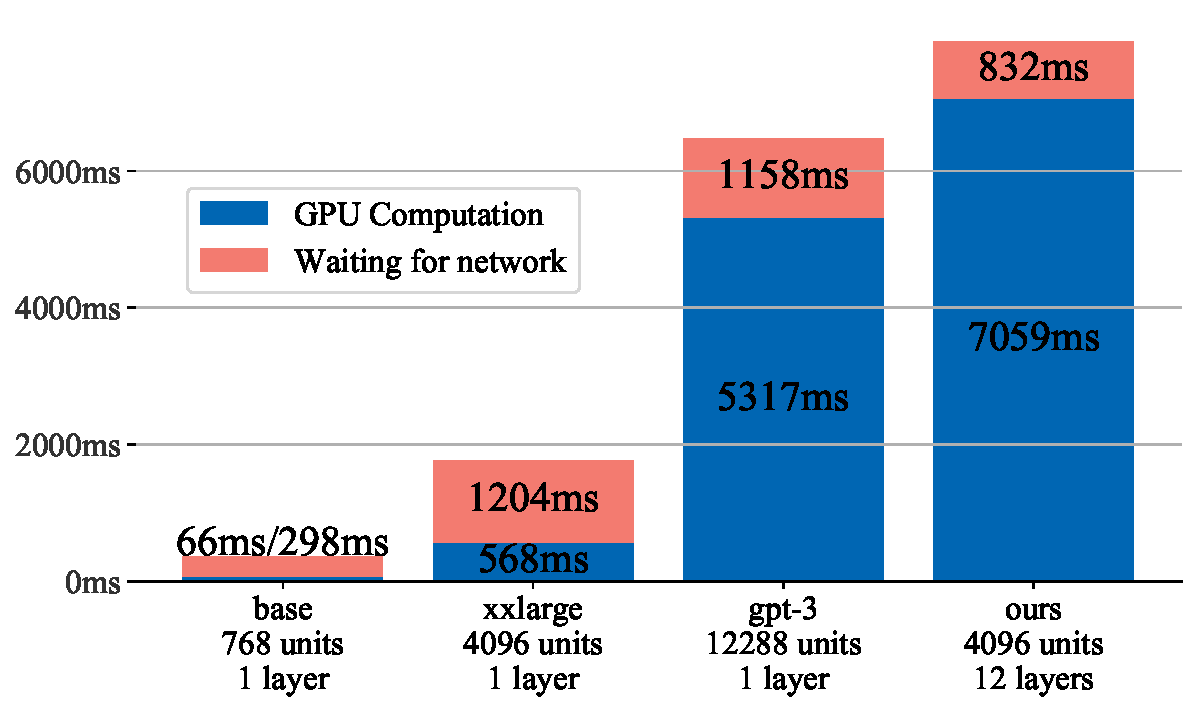
\includegraphics[width=1\linewidth]{resources/perf_absolute.pdf}
    \vspace{-12pt}
    \captionof{figure}{Pipeline computation and idle time per batch at 500 Mb/s bandwidth.}
    \label{fig:throughput_exps}
\end{figure}%
\begin{table}
    \centering
    \captionof{table}{Relative device utilization at 500 Mb/s bandwidth and varying network latency.}
    \label{tab:latency}
    \small
    \setlength{\tabcolsep}{8pt}
    \begin{tabular}[b]{@{}lcccc@{}}
    \toprule
    \multirow{2}{*}{\thead{Latency\\(RTT)}} & 
    \multicolumn{4}{c}{
    \thead{
    Relative GPU utilization\\ (100\% - idle time)
    }
    }
    
    \\
\cmidrule{2-5}                     & base & xxlarge & GPT-3 & Ours \\ \midrule
    None &   18.0\%     &  32.1\%         &  82.1\%  &  89.5\%      \\
    10ms &   11.8\%      &   28.9\%    &   79.3\%   &  87.2\%    \\
    50ms &    4.88\%      &   20.1\%    &   70.3\% &  79.5\%    \\
    100ms &    2.78\%      &    14.9\%    &  60.2\%     &   71.5\% \\
    200ms &   1.53\%     &  10.1\%    &  48.5\%   &     59.2\%    \\
    \bottomrule
    \end{tabular}
    \vspace{-6pt}
\end{table}

As depicted in Figure~\ref{fig:squarecube} (right) and Figure~\ref{fig:throughput_exps}, larger models achieve better GPU utilization rate in the same network conditions, since their communication load grows slower than computation. More importantly, even at 500 Mb/s, the resulting GPU idle time can be pushed into the 10--20\% range, either naturally for GPT-3-sized models or through activation compression for smaller models. In addition, large models maintain most of their training efficiency at the 100ms latency~(Table~\ref{tab:latency}), which is roughly equivalent to training on different continents~\citep{verizon_latency}.

\vspace{-4pt}
\subsection{Detailed Performance Comparison}\label{appendix:training_throughput}

Here we investigate how SWARM parallelism compares to existing systems for training large models: \textbf{GPipe}~\citep{huang2019gpipe} and \textbf{ZeRO-Offload}~\citep{zerooffload}.
The purpose of this section is to compare the training throughput in ``ideal'' conditions (with homogeneous reliable devices and balanced layers), as deviating from these conditions makes it \textit{infeasible} to train with baseline systems.
Still, even in such conditions the performance of different systems can vary across model architectures, and hence we want to identify the cases in which using SWARM is preferable to other approaches.
We benchmark individual SWARM components in preemptible setups in Section~\ref{sect:experiments_adaptive} and Appendix~\ref{appendix:scaling}.

We evaluate training performance for sequences of 4 Transformer layers of identical size distributed over 16 workers. Similarly to Section~\ref{sect:experiments_square_cube}, we use three layer configurations: ``xxlarge''~($d_{model} {=} 4096$, $d_{\text{FFN}} {=} 16384$, 32 heads), ``GPT-3''~($d_{model} {=} 12288$, $d_{\text{FFN}} {=} 49152$, 96 heads), and ``Ours''~($d_{model} {=} 4096$, $d_{\text{FFN}} {=} 16384$, 32 heads, 16 shared layers per block, last stage holds only the vocabulary projection layer). The microbatch size is 4 for ``xxlarge'' and 1 for ``GPT-3'' and ``Ours'', and the sequence length is 512.

To provide a more detailed view of the training performance, we measure two separate performance statistics: the training throughput and the All-Reduce time. 
The training throughput measures the rate at which the system can process training sequences, i.e., run forward and backward passes. 
More specifically, we measure the time required to process 6250 sequences of 512 tokens, which corresponds to the largest batch size used in~\citet{gpt3}.
In turn, the All-Reduce time is the time each system spends to aggregate accumulated gradients across devices. 
Intuitively, training with small batch sizes is more sensitive to the All-Reduce time (since the algorithm needs to run All-Reduce more frequently) and vice versa.


\textbf{Hardware setup:} Each worker uses a V100-PCIe GPU with 16 CPU threads (E5 v5-2660v4) and 128 GB RAM. The only exception is for ZeRO-Offload with ``GPT-3'' layers, where we had to double the RAM size because the system required 190 gigabytes at peak. Similarly to Section~\ref{sect:experiments_square_cube}, each worker can communicate at a 500 Mb/s bandwidth for both upload and download for a total of 1 Gb/s.
In terms of network latency, we consider two setups: with \textbf{no latency}, where workers communicate normally within the same rack, and with \textbf{latency}, where we introduce additional $100\pm50$ms latency directly in the kernel\footnote{More specifically, \texttt{tc qdisc add dev <...> root netem delay 100ms 50ms}}.

\textbf{GPipe configuration:} We use a popular PyTorch-based implementation of GPipe\footnote{The source code is available at \url{https://github.com/kakaobrain/torchgpipe}}. The model is partitioned into 4 stages repeated over 4 model-parallel groups. To fit into the GPU memory for the ``GPT-3'' configuration, we offload the optimizer into RAM using ZeRO-Offload. Before averaging, we use PyTorch's built-in All-Reduce to aggregate gradients.
We evaluate both the standard GPipe schedule and the 1F1B schedule~\citep{pipedream}.

\textbf{ZeRO-Offload configuration:} Each worker runs the entire model individually, then exchanges gradients with peers. For ``xxlarge'', we use the official implementation from~\cite{zerooffload}. However, for ``GPT-3'', we found that optimizer offloading still does not allow us to fit 4 layers into the GPU. For this reason, we also offload the model parameters using the \texttt{offload\_param} option.

\begin{table}
\centering
\small
\setlength{\tabcolsep}{4pt}
\captionof{table}{Training performance for different model sizes.}
\label{tab:throughput_gpt}
\begin{tabular}[b]{lcccc}
\toprule
\multirow{2}[2]{*}{System} &
  \multicolumn{2}{c}{Throughput, min/batch} &
  \multicolumn{2}{c}{All-Reduce time, min} \\ \cmidrule(lr){2-3}\cmidrule(lr){4-5} 
                 & No latency & Latency & No latency & Latency \\
 \midrule \multicolumn{5}{c}{``GPT-3'' (4 layers) }\\
 \midrule
SWARM            &  168.3 &\textbf{186.7}  &  7.4 & \textbf{7.6}   \\
GPipe            &  164.5 & 218.4 &  \multirow{2}{*}{\textbf{6.7}}    & \multirow{2}{*}{7.8}   \\
1F1B & \textbf{163.3} & 216.1 & & \\
Offload          &  272.7 & 272.7          &  25.5 & 27.3 \\
\midrule \multicolumn{5}{c}{``xxlarge'' (4 layers) }\\
\midrule
SWARM            &  44.2 & 48.2                  &  0.8  & \textbf{0.9}   \\
GPipe            &  40.1 & 108.8                  &  \multirow{2}{*}{\textbf{0.7}}  & \multirow{2}{*}{1.1}   \\
1F1B & 40.8 & 105.5 & & \\
Offload          &  \textbf{33.8} & \textbf{33.8}  &  2.8 & 4.2   \\
\midrule \multicolumn{5}{c}{Full ``Ours'' model (48 shared layers + embeddings) }\\
\midrule
SWARM            &  432.2 & 452.9                  &  0.8  &\bf 1.0   \\
GPipe            &  420.0 & 602.1                   &  \multirow{2}{*}{\bf 0.7}  & \multirow{2}{*}{1.1}   \\
1F1B             &  408.5 & 569.2 & & \\
Offload          &  \bf 372.0 &\bf 372.0  &  3.2 & 4.8   \\
\bottomrule
\end{tabular}
\vspace{-8pt}
\end{table}%

\begin{figure}[b]
\vspace{-16pt}
\centering
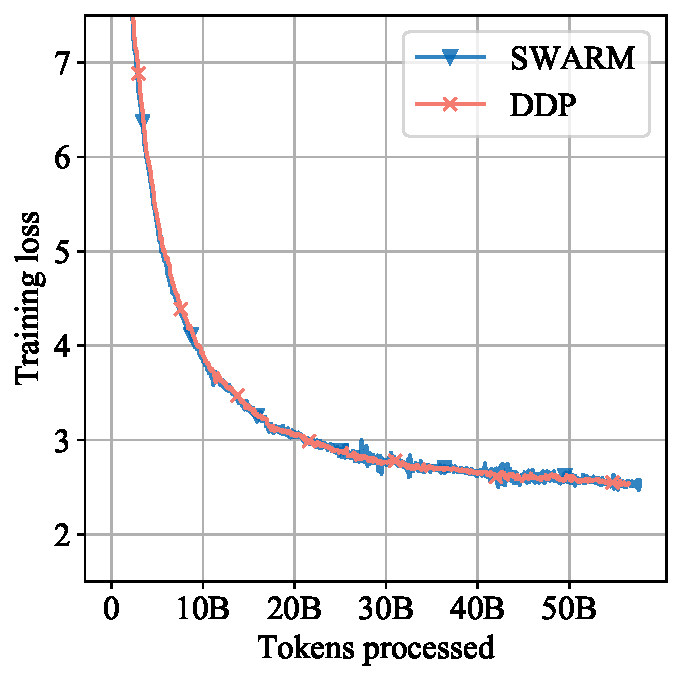
\includegraphics[ width=0.65\linewidth]{resources/learning_3stages.pdf}
\vspace{-6pt}
\captionof{figure}{Training convergence comparison.}
\label{fig:convergence}
\end{figure}

In turn, when training smaller models, ZeRO-Offload outperforms both SWARM and GPipe. This result aligns with our earlier observations in Figure~\ref{fig:squarecube}, where the same model spent most of the time waiting for the communication between pipeline stages.%

We also observe that ZeRO-Offload takes longer to aggregate gradients, likely because each peer must aggregate the entire model, whereas in SWARM and GPipe, peers aggregate a single pipeline stage. The variation between All-Reduce time in GPipe and SWARM is due to implementation differences. Overall, SWARM is competitive to HPC baselines even in an idealized homogeneous environment.

\subsection{Large-Scale Distributed Training}
\label{sect:experiments_large}

To verify the efficiency of SWARM parallelism in a practical scenario, we conduct a series of large-scale distributed experiments using preemptible (unreliable) cloud T4 and A100 GPUs over a public cloud network.

We train a Transformer language model with the architecture similar to prior work~\citep{gpt3,gptj,gptneo} and 1.01 billion parameters in total. Our model consists of 3 stages, each containing a single Transformer decoder block with $d_{model}=4096$ and 16 layers per pipeline stage. All workers within a stage serve the same group of layers, and all layers within each group use the same set of parameters, similarly to ALBERT~\citep{albert}. On top of this, the first stage also contains the embedding layer, and the last stage includes the language modeling head. Because of layer sharing, this model is equivalent to a 13B model from~\citet{gpt3} in terms of compute costs. 

We use 8-bit compression~\citep{adam8bit} for activations and gradients to reduce the communication intensity. Additional training setup details are covered in Appendix~\ref{appendix:detailed_large}.
SWARM nodes run rebalancing every $T=300$ seconds, and trainers measure peer performance using a moving average with $\alpha=0.1$. However, as we show in Section~\ref{sect:experiments_adaptive}, the throughput of SWARM is not very sensitive to the choice of these hyperparameters.



First, to verify that model parallelism with asynchronous updates does not have significant convergence issues, we train the model on the Pile~\citep{gao2020pile} dataset with 400 preemptible T4 instances, each hosting one accelerator. As a baseline, we use regular data-parallel training with offloading on 128 A100 GPUs.
We run both experiments for approximately 4 weeks and compare the learning curves.




Figure~\ref{fig:convergence} shows the results of this experiment: it can be seen that the training dynamics of two approaches are indeed similar, which demonstrates the viability of SWARM parallelism for heterogeneous and poorly-connected devices.

In the next experiment, we aim to measure the pipeline throughput in different hardware conditions and to compare it with an estimate of best-case pipeline performance.
We consider several setups: first, we use the same 400 preemptible T4 nodes; in another setup, we use 7 instances with 8 A100 GPU each; finally, we combine these fleets to create a heterogeneous setup. We examine the performance of the pipeline both with weight sharing and with standard, more common, Transformer blocks.

\begin{table}
\centering
\captionof{table}{Pipeline throughput, layer sharing.}
\label{tab:throughput}
\small
\begin{tabular}{@{}lcccc@{}}
\toprule
\multirow{2}{*}{\begin{tabular}[c]{@{}l@{}}Hardware\\ setup\end{tabular}} &
  \multicolumn{2}{c}{\begin{tabular}[c]{@{}c@{}}Throughput,\\ samples/s\end{tabular}} &
  \multicolumn{2}{c}{\begin{tabular}[c]{@{}c@{}}Optimal\\ bandwidth, Mb/s\end{tabular}} \\ \cmidrule(lr){2-3}\cmidrule(lr){4-5} 
                 & Actual & Best-case & Upload & Download \\ \midrule
T4           &  17.6      &   19.2        &   317.8     &     397.9     \\
A100          & 16.9       &   25.5        &   436.1     &     545.1     \\
T4 \& A100 &   27.3     &       ---    &   ---     &      ---    \\ \bottomrule
\end{tabular}
\end{table}
\begin{table}
\centering
\captionof{table}{Pipeline throughput, default Transformer.}
\label{tab:throughput_standard}
\small
\begin{tabular}{@{}lcc@{}}
\toprule
\multirow{2}{*}{\begin{tabular}[c]{@{}l@{}}Hardware\\ setup\end{tabular}} &
  \multicolumn{2}{c}{\begin{tabular}[c]{@{}c@{}}Throughput,\\ samples/s\end{tabular}} \\ \cmidrule(lr){2-3}
                 & Actual & Best-case \\ \midrule
T4           &  8.8      &   19.3        \\
A100          & 8.0       &   25.1        \\
T4 \& A100 &   13.4     &       ---    \\ \bottomrule
\end{tabular}
\end{table}






We measure the number of randomly generated samples processed by the pipeline both in our infrastructure and the ideal case that ignores all network-related operations (i.e., has infinite bandwidth and zero latency). The ideal case is emulated by executing a single pipeline stage 3 times locally on a single server and multiplying the single-node estimates by the number of nodes.

As demonstrated in the left two columns of Table~\ref{tab:throughput} and Table~\ref{tab:throughput_standard}, asynchronous training of compute-intensive models with 8-bit compressed activations regardless of the architecture specifics allows us to achieve high performance without a dedicated networking solution. Furthermore, the load balancing algorithm of SWARM allows us to dynamically and efficiently utilize different hardware without being bottlenecked by slower devices. 


Next, we use the same load testing scenario to estimate the bandwidth required to fully utilize each device type in the above infrastructure. For this, we measure the average incoming and outgoing bandwidth on the nodes that serve the intermediate stage of the pipeline. We summarize our findings in the right two columns of Table~\ref{tab:throughput}: it turns out that with layer sharing and 8-bit compression, medium-performance GPUs (such as T4) can be saturated even with moderate network speeds. Based on our main experiment, the optimal total bandwidth is roughly 100Mb/s higher than the values reported in Table 3 due to gradient averaging, loading state from peers, maintaining the DHT and streaming the training data.
Although training over the Internet with more efficient hardware might indeed underutilize the accelerator, this issue can be offset by advanced compression strategies such as compression-aware architectures or layer sharing, as shown in Table~\ref{tab:throughput}.

\begin{figure}[t]
    \centering
    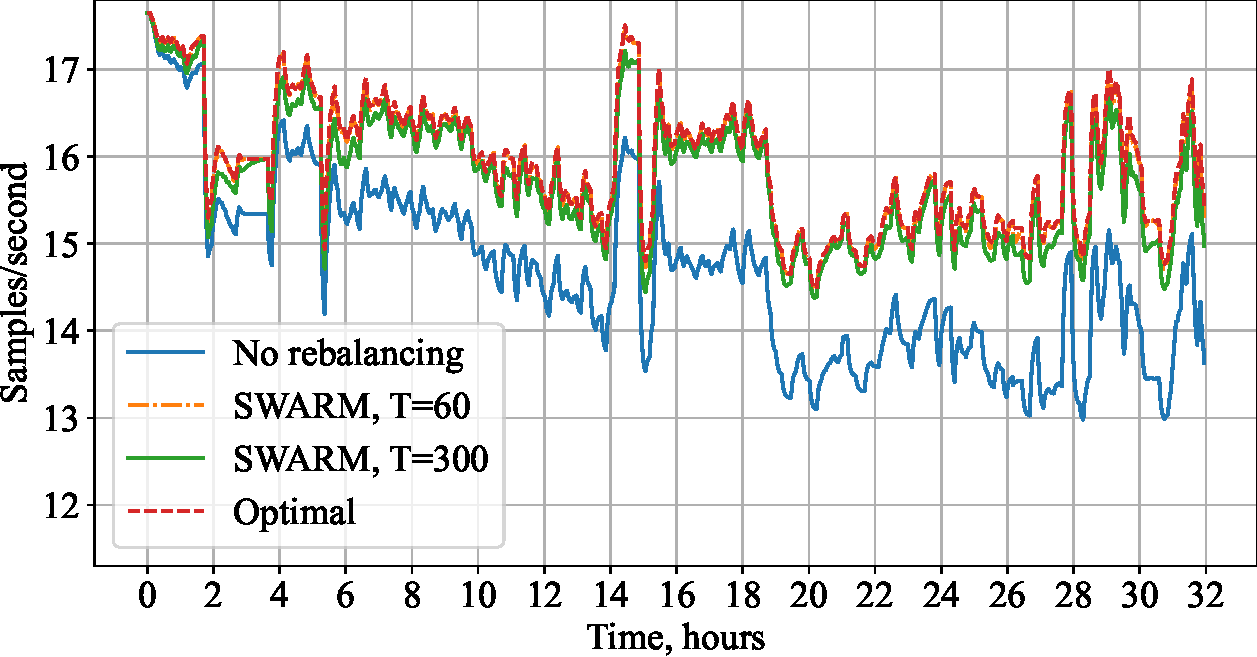
\includegraphics[width=\linewidth]{resources/rebalancing_activity.pdf}
    \captionof{figure}{Throughput of rebalancing methods over time.}
    \label{fig:rebalancing}
\end{figure}

\subsection{Adaptive Rebalancing Evaluation}


\begin{figure*}[h!]
\begin{subfigure}{0.5\textwidth}
    \centering
    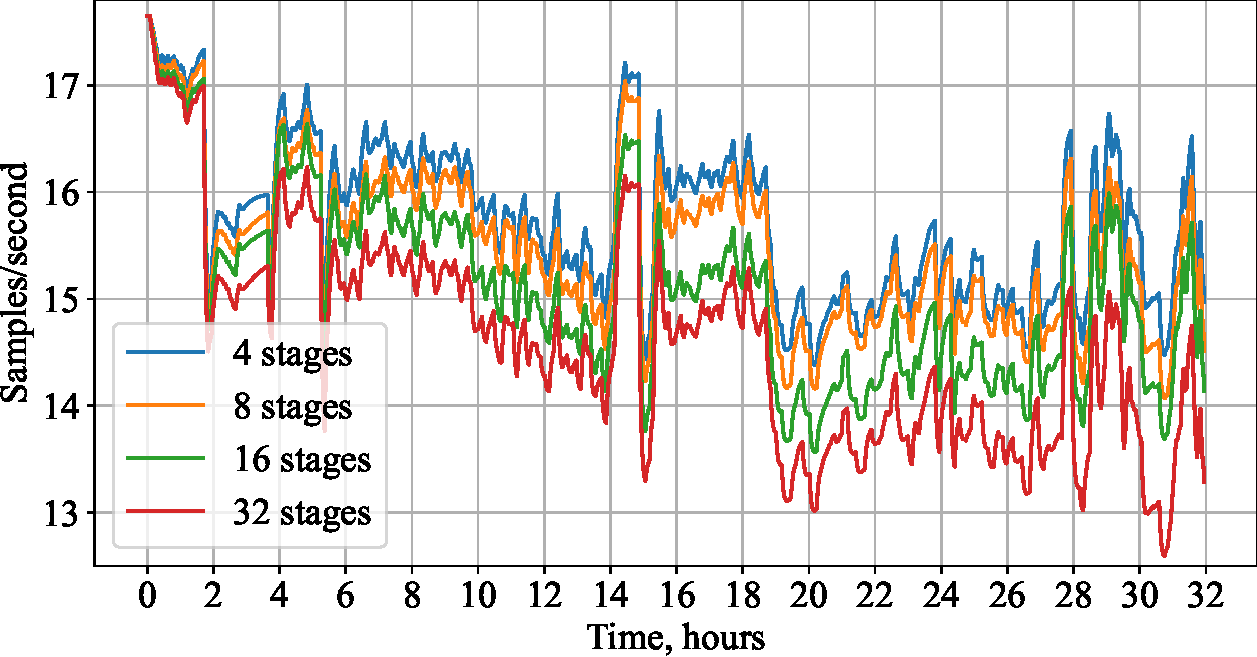
\includegraphics[width=0.97\linewidth]{resources/rebalancing_stages.pdf}
    \caption{Adaptive rebalancing of SWARM parallelism.}
    \label{fig:rebalancing_stages}
\end{subfigure}%
\begin{subfigure}{0.5\textwidth}
    \centering
    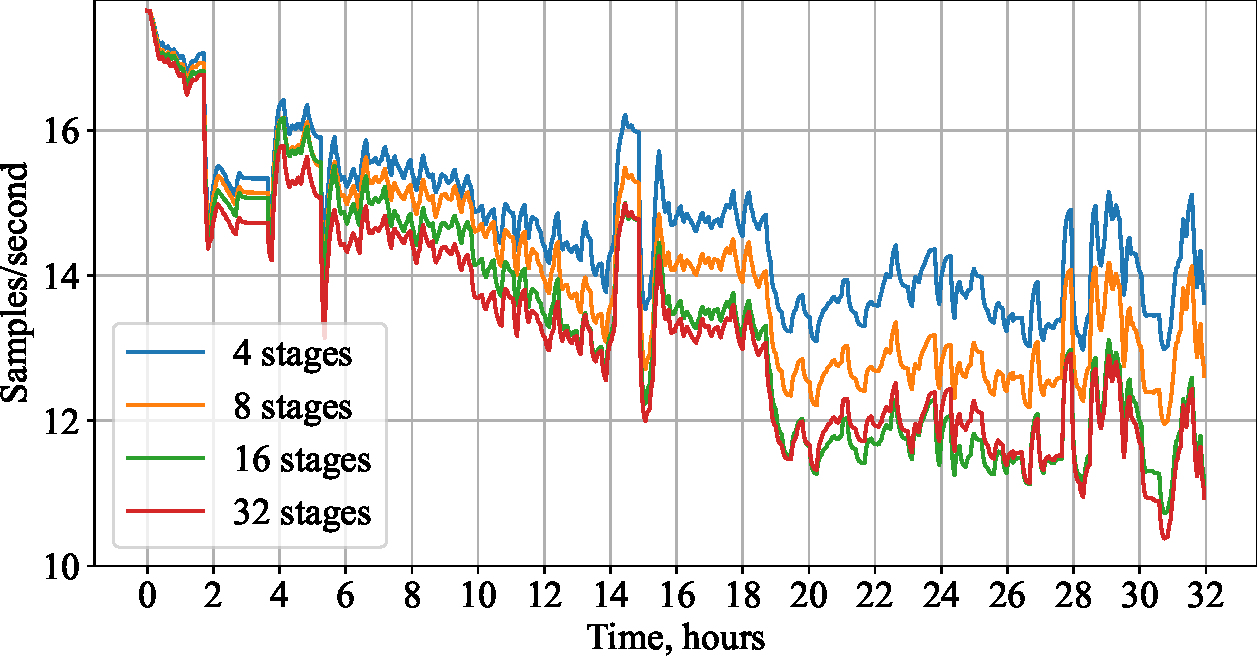
\includegraphics[width=0.97\linewidth]{resources/rebalancing_stages_baseline.pdf}
    \caption{No rebalancing.}
    \label{fig:rebalancing_stages_baseline}
\end{subfigure}
\caption{Scaling of pipeline-parallel strategies with respect to the number of stages.}
\label{fig:rebalancing_stages_all}
\end{figure*}

\label{sect:experiments_adaptive}
In this experiment, we evaluate the efficiency of adaptive peer rebalancing between stages proposed in Section~\ref{sect:method_swarm}. 
We use statistics of the number of active T4 nodes from the 32-hour segment of the experiment described in Section~\ref{sect:experiments_large}. 
We use this data to simulate training dynamics by viewing it as sequence of events, each consisting of a timestamp and a change in the number of peers (which can be positive or negative). 
When a worker is removed from the pipeline, we randomly choose the stage it was removed from: that is, removing $N$ peers corresponds to $N$ samples from the uniform distribution over four pipeline stages. 
We run 10 simulations with different random seeds and average the resulting trajectories.
We compare our strategy with two different values of $T$ to the baseline that has no rebalancing.

The results of this evaluation are available in \autoref{fig:rebalancing}; for reference, we also provide the performance of a theoretically optimal rebalancing strategy that maintains the highest possible throughput at every moment. It can be seen that even with the rebalancing period $T=300$, our approach significantly improves the overall throughput of the pipeline. When the number of peers is relatively stable, the rebalanced pipeline also approaches the optimal one in terms of throughput, which shows the efficiency of rebalancing even when moving only one node at a time.

In addition, we observed that for some brief periods, the performance of the unbalanced pipeline exceeded the throughput of the balanced one due to random choice of disconnecting peers (dropping more from the ``overrepresented'' stages affects the imbalanced pipeline less). However, this held true only for $\approx 4.5\%$ of the experiment and was quickly mitigated by adaptive rebalancing.

As expected, decreasing $T$ from 300 to 60 seconds improves both the overall throughput and the speed of convergence to optimal pipeline performance. However, the effect is not as drastic compared to the increase in DHT data transfer volume. This is also demonstrated by \autoref{tab:rebalancing_speedup}, which shows the relative throughput of the three configurations compared to the optimal one. Furthermore, the table displays that while initially there is little difference between rebalancing choices, it becomes more pronounced later on as the imbalanced version ``drifts further'' from the optimal state.

\begin{table}[b]
\centering
\captionof{table}{Relative throughput comparison of pipeline rebalancing methods.}
\small
\label{tab:rebalancing_speedup}
\begin{tabular}[b]{@{}lccc@{}}
\toprule
\multirow{2}[2]{*}{\thead{Rebalancing}} & \multicolumn{3}{c}{\% of optimal} \\ \cmidrule(l){2-4} 
                        & Overall   & First 1 hour   & Last 1 hour  \\ \midrule
None                & 82.7      & 99.0       & 45.4     \\
$T=300$    & 95.8      & 99.4       & 88.9     \\
$T=60$     & 97.6      & 99.8       & 91.7     \\ \bottomrule
\end{tabular}
\end{table}

Finally, we analyze the scaling properties of rebalancing with respect to the number of stages. To do this, we conduct experiments in the same setup as above ($T=300$) while changing the number of pipeline stages from 4 to $\{4,\ 8,\ 16,\ 32\}$. To ensure the consistency of throughput across all experiments, we increase the starting number of peers accordingly while keeping the preemption rate constant. As a baseline, we also evaluate the throughput of the pipeline that has no rebalancing.

Figure~\ref{fig:rebalancing_stages_all} shows the outcome of this experiment. As displayed in the plots, both strategies drop in performance with the increase in the stage count: while all stages should drop in performance equally in expectation, in practice, the variances are too large while the number of peers is relatively too small for the asymptotic properties to take place. This effect results in more outliers (large drops in the number of peers) in the preemption distribution for more stages. Still, rebalancing allows to partially mitigate the issue: while we observe a more consistent downward trend for the baseline strategy, the rebalanced pipeline regains its performance over time and achieves a higher overall throughput.



\section{Conclusion}
In this work, we advance the method of {machine unlearning} through a novel viewpoint: model sparsification, achieved by weight pruning. We show in both theory and practice that model sparsity plays a foundational and crucial role in closing the gap between exact unlearning and existing approximate unlearning methods. Inspired by that, we propose two new unlearning paradigms,  `prune first, then unlearn' and `sparsity-aware unlearn', which can significantly improve the efficacy of approximate unlearning. We demonstrate the effectiveness of our findings and proposals in extensive experiments across different unlearning setups. Our study also indicates the presence of \textit{model modularity} traits, such as weight sparsity, that could simplify the process of machine unlearning. This may open up exciting prospects for future research to investigate unlearning patterns within weight or architecture space.






\pagebreak



\bibliographystyle{icml2023}
\bibliography{bibliography}

\clearpage
\appendix
\section*{Supplementary Material}

This part of the paper is organized as follows:
\begin{itemize}
    \item \cref{appendix:faq} overviews several common questions about the details of our study and addresses the limitations of SWARM parallelism;
    \item In \cref{appendix:related}, we list further related works on topics relevant to the problem setting we study;
    \item In \cref{appendix:wiring_details} and \cref{appendix:rebalancing_formal}, we give a more formal description and outline the details of stochastic wiring and adaptive rebalancing, accordingly;
    \item In \cref{appendix:equivalence}, we outline the relation between training with SWARM and using methods for offloading.
    \item \cref{appendix:detailed_setup} and  \cref{appendix:detailed_large} contain additional details of our experimental setup, whereas \cref{appendix:scaling} reports further experiments on specific aspects and components of SWARM parallelism;
    \item Lastly, we investigate compression-aware architectures in \cref{appendix:compression} and evaluate their impact in a practical setting in \cref{appendix:time_to_solution}.
\end{itemize}

\section{Answers to Common Questions}
\label{appendix:faq}


\paragraph{Why not just use data parallelism with offloading?}

Regular data parallelism requires all-reduce steps where peers exchange gradients, which can be prohibitively expensive for large models. For example, a 1 billion parameter model with 16-bit gradients requires 2 GB of data to be synchronized between all $n$ devices. We need at least $n$ messages to perform this synchronization. If we have 100 devices with bidirectional communication, each client would need to send 2 GB of data to finish the synchronization. Thus, with slow interconnects, such synchronizations are not practical.

\paragraph{Why not just use fully sharded data parallelism with elasticity?}

Sharded data parallelism requires all-to-all communication of parameter buffers at each layer. Each of these communications can be done in parallel and has a size of parameter count divided by $n$; in total, $n$ messages are required. Thus, for 1B parameters in 16-bit precision, a total of 2 GB need to be synchronized for both the forward and backward pass. For low-bandwidth devices with 100 Mb/s speed, this would entail an overhead of 5.5 minutes per forward/backward pass, which is difficult to overlap with computation. This is exacerbated further, because all-to-all communication latency is determined by the slowest peer. Thus, sharded data parallelism can be particularly inefficient for setups where peers have different network bandwidths.

\paragraph{Should I use SWARM in a supercomputer?}
By default, SWARM is worse than traditional parallelism due to its extra complexity (see experiments in Section~\ref{appendix:training_throughput}). However, SWARM can be useful in case of supercomputers that have heterogeneous devices.

\paragraph{ZeRO-Offload allows one to train 13B parameters on a single V100, so why do I need SWARM?}

Using ZeRO-Offload can slow down training due to the slow data transfer between external memory and the accelerator. Training with SWARM can {\it accelerate} training while also allowing to train larger models; see Appendix~\ref{appendix:equivalence} for a detailed comparison.

\paragraph{Is it worth using preemptible instances and SWARM from an economic standpoint?}
Due to a significantly smaller cost per hour, one can leverage a larger amount of computation when using spot instances compared to on-demand cloud VMs or dedicated HPC setups. See \autoref{appendix:time_to_solution} and \autoref{tab:cost} for a comparison of both hourly and total costs for an example large-scale pretraining task.

\paragraph{When should I avoid using SWARM?}

SWARM is efficient at training compute-intensive models with more than 1B parameters. For smaller models, a sharded data-parallel approach can be more optimal. For homogeneous HPC environments, standard sharded data-parallel or pipeline-parallel training will be more efficient than SWARM, because the rebalancing is not required. For HPC environments that are so extensive that the failure of a node is likely, the practicality of SWARM depends on how many nodes are expected to fail. Elastic sharded data parallelism is better than SWARM if the number of expected failures is relatively low.

\paragraph{Can I use SWARM without layer sharing or quantization?}
Yes, SWARM can still be effective in these scenarios. Our bandwidth experiments in the main part of the work give an estimate of its network overhead. By using no quantization, which means using regular 16-bit activations, the network overhead increases approximately by a factor of two. Without layer sharing, the overhead within each pipeline stage to synchronize the gradients is increased by the number of layers not being shared. As such, a rough estimate of the efficiency of SWARM in these scenarios can be estimated by taking our model size and network bandwidth requirements data and multiplying it by the relevant factor.

\paragraph{Do the compression-aware architecture modifications apply only to Transformers?} 
Bottleneck and maxout compression are general compression techniques that can be applied to any layer in any architecture. However, their effectiveness may vary depending on where in the model they are applied and what kind of model these are applied to (for example, CNNs vs. RNNs vs. Transformers).

\paragraph{How many pipeline stages can SWARM have?}
While its design allows for any number of stages, using long pipelines can result in a reduced training throughput. Similarly to regular pipeline parallelism, SWARM suffers from the pipeline ``bubble'' problem~\citep{huang2019gpipe}: at the beginning of the initial batch processing, peers near the end of the pipeline will be waiting for inputs. Likewise, early layers will be idle after processing the final microbatch.
In theory, this can be mitigated with asynchronous updates~\citep{pipedream,pipemare}, but we did not investigate them in this work due to potential convergence issues.

\paragraph{How much failure can SWARM handle?}
As long as there is at least one operational peer at every pipeline stage and at least one trainer, SWARM can work without any issues. 
The key factors defining the training run state at a given SGD step are the model parameters, the optimizer statistics, the data loader state, and the step number (required for proper scheduling). The up-to-date parameters and optimizer statistics, as well as the step number, are naturally located on all active nodes of a given stage, since they are required for training. Thus, when a peer joins the network, it can download the checkpoint corresponding to the current training state from other peers.

As we mention in Section~\ref{sect:method_swarm}, peer failures do not affect forward and backward passes as long as there is at least one peer at the required stage: because of rewiring, it is possible to resend activations or gradients to another worker that has identical model weights by construction. Similarly, the data loader state can be recomputed from the last known SGD step. However, we do not track the order of examples sampled within the same batch; because of the i.i.d. assumption in the large-scale training setup, the distribution of gradients is expected to be the same. Hence, if the peer leaves from the pipeline stage, other workers can compute gradients and replace those accumulated by the disconnected peer, so that the number of examples for an SGD step stays the same.

\paragraph{Some configurations in Section~\ref{sect:experiments_square_cube} measure less than $\bf 20\%$ GPU idle time, while many HPC systems only achieve $\bf \approx80\%$ GPU utilization. Does this mean that SWARM is $\bf 30\%$ faster?} 
No, because these are different measurement types. \citet{megatron2} measures GPU utilization as a fraction of theoretical peak FLOP/s of their GPUs. In contrast, we only measure what fraction of time the GPU is running the model, regardless of efficiency. Since any realistic deep learning workload cannot achieve $100\%$ peak FLOP/s, $20\%$ GPU idle time for SWARM means that it can reach $\approx0.8$x the training throughput compared to training with an infinitely fast network. As a rule of thumb, one can say that SWARM will run at a $20\%$ slower speed than systems described by~\citet{megatron2} using the infrastructure that is several times cheaper.%


   



\section{Additional Related Work}\label{appendix:related}


\vspace{-2pt}
\paragraph{Dynamic parameter loading.} Several recent studies propose alternative execution algorithms that allow training large models with data parallelism. Since neural networks typically use a small fraction of weights at any given moment, the remaining ``inactive'' parameters can be sharded~\citep{zero} or offloaded to external memory~\citep{l2l,zerooffload,zero_ssd}. In sharded data parallelism~\cite{zero}, inactive tensors are distributed across all $n$ devices such that each device stores $\frac{1}{n}$th of all parameters. For active layers, the shards are gathered such that each device holds the entire tensor just-in-time for computation. After the computation, the parameters' memory is freed so that only the sharded memory remains ($\frac{1}{n}$th per device). This makes it very memory efficient to store model and optimizer states for inactive layers if many devices are available. Similarly to tensor parallelism, these algorithms can support arbitrary models without the need for layer partitioning and can, in principle, run a large model on a single GPU, which is useful for finetuning and inference.

\vspace{-6pt}
\paragraph{Architecture-specific methods.} Finally, some distributed training algorithms take advantage of specific layers, such as locally connected layers~\citep{dean12,coates13}, Mixture-of-Experts~\citep{moe_first,shazeer2017outrageously,Lepikhin2020GShardSG}, Switch layers~\citep{fedus2021switch} or Product Key Memory~\citep{pkm}. These layers contain many near-independent parts that can be assigned to different devices. They can easily scale to an extremely large number of parameters with a relatively small increase in compute~\citep{shazeer2017outrageously}. However, they are also less parameter-efficient~\citep{fedus2021switch} and may not apply to all architectures.

\vspace{-6pt}
\paragraph{Optimal scheduling for distributed training.}
When the configuration of each peer is known, it is possible to significantly optimize the pipeline scheduling by going beyond the greedy approach with global optimization techniques~\citep{alpa,piper}, even with heterogeneous hardware~\citep{yuan2022decentralized}.
However, we consider a setup in which this is not possible: preemptible and volunteer peers can join at any point of the experiment, and dynamically rescheduling and orchestrating them in a centralized manner is technically difficult because of the communication and reliability constraints.

\vspace{-6pt}
\paragraph{Elastic training.} To train with a dynamic number of workers, deep learning practitioners have developed elastic training algorithms~\citep{pytorch_elastic,elastic_horovod}. If a worker leaves or fails during training, these algorithms rebalance the load between the remaining nodes and continue the training procedure~\citep{proteus,moshpit}. If new workers join during training, they get the latest model parameters from their peers and train alongside them.

\vspace{-10pt}
\paragraph{Asynchronous training.} Another important problem is distributed training on devices with uneven performance. One way to solve this problem is to use asynchronous training, where nodes compute gradients at their own pace and aggregate them using a parameter server~\citep{recht2011hogwild,volunteer_dl_async} or a decentralized network~\citep{dp_sgd}. This idea allows full utilization of each device, but may reduce the convergence rate due to ``stale'' gradients~\citep{recht2011hogwild,aji2019making}. Several studies~\citep{wagma,moshpit,zerooffload,dedloc} propose hybrid techniques that remove some synchronization points while maintaining the per-iteration convergence.


\section{Stochastic Wiring Details}\label{appendix:wiring_details}

Our approach uses \textit{stochastic wiring}, a specialized routing algorithm designed around heterogeneous unreliable devices and high network latency. The core idea of stochastic wiring is to route each training microbatch through random devices from each pipeline stage, such that the workload of each device is proportional to its performance.
The performance of the peer is measured as an exponentially weighted average of its response time, and all peers serving a specific stage are stored in a priority queue. 
We formally describe the components of stochastic wiring in Algorithm~\ref{alg:wiring}.

From a system design perspective, each worker runs a separate \textit{trainer} process that forms microbatches and routes them through pipeline stages (forward and backward pass). As we describe earlier in Section~\ref{sect:method_swarm}, trainers run Interleaved Weighted Round Robin~\citep{iwrr,interleaved_round_robin} (IWRR) scheduling to dynamically assign microbatches to peers based on each peer's training throughput (``samples per second'') in a balanced way.


An important observation is that \textit{stochastic wiring allows SWARM to mitigate network latency}. Unlike existing pipeline algorithms~\citep{huang2019gpipe}, SWARM workers do not get blocked if their neighbors take too long to process a minibatch. Instead, each SWARM device maintains a queue of microbatches assigned by trainers. In case of a latency spike, workers keep processing previously queued microbatches, maintaining high device utilization.

\begin{figure}[t]
\vspace{-1em}
\begin{algorithm}[H]
  \captionof{algorithm}{Pseudocode of stochastic wiring}
  \label{alg:wiring}
\begin{algorithmic}[1]
  \INPUT the number of pipeline stages $N$, the set of active servers $S$, smoothing parameter $\gamma$, initial priority $\epsilon$

  \STATE \(\triangleright\) Initialization
  \STATE ema = dict()
  \STATE queues = list()
  \FOR{$\text{i} \in 1,\ldots, N$}
  \STATE queues.append(PriorityQueue())
  \ENDFOR
  \STATE \textbf{def} add\_server(server)\textbf{:}
      \STATE \hspace{12px} ema[server] = $\varepsilon$
      \STATE \hspace{12px} \textbf{for} $\text{i} \in \text{get\_blocks\_served\_by(server)}$\textbf{:}
        \STATE \hspace{24px} queues[i].update(server, priority=$\varepsilon$)
  \STATE \textbf{def} ban\_server(server) \textbf{:}
      \STATE \hspace{12px} \textbf{for} $\text{i} \in \text{get\_blocks\_served\_by(server)}$\textbf{:}
        \STATE \hspace{24px} queues[i].update(server, priority=$\infty$)
  \STATE \textbf{def} choose\_server(i)\textbf{:}
      \STATE \hspace{12px} server, priority = queues[i].top()
      \STATE \hspace{12px} new\_priority = priority + ema[server]
      \STATE \hspace{12px} \textbf{for} $\text{j} \in \text{get\_blocks\_served\_by(server)}$ \textbf{:}
          \STATE \hspace{24px} queues[j].update(server, priority=new\_priority)
      \STATE \hspace{12px} \textbf{return} server
  \STATE \(\triangleright\) Forward pass with stochastic wiring
  \STATE \textbf{def} forward(inputs):
      \STATE \hspace{12px} layer\_index = 0
      \STATE \hspace{12px} \textbf{while} $\text{layer\_index} < N$\textbf{:}
          \STATE \hspace{24px} server = choose\_server(layer\_index)
          \STATE \hspace{24px} t = get\_current\_time()
          \STATE \hspace{24px} \textbf{try:}
          \STATE \hspace{36px} inputs = server.forward(inputs)
          \STATE \hspace{36px} layer\_index = layer\_index + 1
          \STATE \hspace{36px} $\Delta t$ = get\_current\_time() - t
          \STATE \hspace{36px} ema[server] = $\gamma \cdot \Delta t + (1 - \gamma) \cdot$ ema[server]
          \STATE \hspace{24px} \textbf{catch} (ServerFault, Timeout):
          \STATE \hspace{36px} ban\_server(server)
      \STATE \hspace{12px} \textbf{return} inputs
\end{algorithmic}
\end{algorithm}
\vspace{-25pt}
\end{figure}

\section{Description and Complexity of Adaptive Rebalancing}
\label{appendix:rebalancing_formal}

Algorithm~\ref{alg:adaptive_rebalancing} contains the formal definition of the adaptive rebalancing procedure. As described previously, each worker of SWARM that hosts model layers continuously updates the information about its load in parallel with processing the incoming requests. Each $T$ seconds, the peers measure the total load for all stages of the pipeline, and the peer with the lowest queue size from the stage with the minimum load moves to the stage with the maximum load. In principle, the algorithm could be extended to support moving multiple peers simultaneously; however, as we have shown in Section~\ref{sect:experiments_adaptive}, even in the current form the algorithm bridges most of the gap between the optimally balanced pipeline and the system without any rebalancing.

The complexity of Algorithm~\ref{alg:adaptive_rebalancing} can be estimated as follows: for $M$ as the highest number of peers over all stages, we have $O(M)$ operations in Lines 9--11 and Lines 22--24, and all other operations take constant time for a single stage. These operations are nested in the loop over all stages, which means that the total complexity of the algorithm is $O(MS)$. For practical numbers of both peers (e.g., < 10,000) and stages (fewer than 100), this incurs a negligible overhead on performance, as all communication and computation is done in parallel with the actual forward and backward passes.

Also, notice that only one migrating peer needs to stop processing requests and download the weights and optimizer statistics of the pipeline stage it starts serving: this means that the overall network load of this procedure is relatively small, as all DHT requests handle scalar data and do not exceed the number of active peers for each worker.

In practice, the algorithm handles slight deviations in local time and network/DHT latencies by allowing the peers to wait for straggling nodes in Line 9 for a predefined timeout. If a node does not join the rebalancing procedure by reporting its load in time or joins the network too late, it is omitted from the current iteration. 



\begin{algorithm}
  \caption{Adaptive rebalancing for SWARM parallelism}
  \label{alg:adaptive_rebalancing}
\begin{algorithmic}[1]
  \INPUT peer index $i$, current peer stage $s_{cur}$, total number of stages $S$, rebalancing period $T$
  \WHILE{active}
  \STATE Sleep for $T$ seconds
  \STATE Measure $q_i$ as the local request queue size
  \STATE Write $(i, q_i)$ as the key-subkey pair to DHT[$s_{cur}$]
  \STATE Initialize minimum and maximum load stages: $s_{min}=s_{max}:=-1$,
  \STATE $l_{min}:=\infty, l_{max}:=-\infty$
  \FOR{$s$ in $1,\ldots, S$}
  \STATE Initialize the load buffer $L = 0$
  \FOR{$(j,q_j)$ in DHT[$s$]}
  \STATE $L:=L+q_j$
  \ENDFOR 
  \IF{$L>L_{max}$}
  \STATE $s_{max}:=s,\ L_{max}:=L$
  \ENDIF
  \IF{$L<L_{min}$}
  \STATE $s_{min}:=s,\ L_{min}:=L$
  \ENDIF
  \ENDFOR
  \IF{$s_{cur}=s_{min}$}
  \STATE // Migrate to the maximum load stage
  \STATE Initialize the minimum load peer $i_{min}:=-1,q_{min}:=\infty$
  \FOR{$(j,q_j)$ in DHT[$s$]}
  \IF{$q_j<q_{min}$}
  \STATE $i_{min}:=j,\ q_{min}:=q_j$
  \ENDIF
  \ENDFOR
  \IF{$i_{min}=i$}
  \STATE // This peer should migrate
  \STATE $s_{cur}:=s_{max}$
  \STATE Download up-to-date parameters from peers in $s_{max}$
  \ENDIF
  \ENDIF
  \ENDWHILE
\end{algorithmic}
\end{algorithm}

\section{Relation between SWARM and ZeRO-Offload}\label{appendix:equivalence}
\vspace{2pt}

In this section, we argue that depending on the use of DPU, SWARM-parallel training is equivalent to either fully synchronous training or the semi-synchronous training proposed in ZeRO-Offload~\citep{zerooffload}.
That is, SWARM produces exactly the same stepwise updates as conventional distributed training algorithms and will therefore achieve a solution in the same number of steps.

\vspace{2pt}

This observation is similar to how many advanced distributed training techniques~\citep{huang2019gpipe,zero} are computationally equivalent to regular synchronous training on a single device. For instance, despite using advanced distributed computation strategies, GPipe~\citep{huang2019gpipe} computes exactly the same mathematical expression to obtain gradients and applies those gradients in the same order as any other \textit{synchronous} training algorithm. On the other hand, PipeDream~\citep{pipedream} changes the order in which the updates are applied, introducing the so-called stale gradients~\citep{recht2011hogwild}. This allows PipeDream to improve device utilization but has been shown to reduce the final model quality in some setups~\citep{MLSYS2020_96da2f59}.

\vspace{2pt}

Despite using randomized routing and asynchronous communication between pipeline stages, SWARM still performs optimizer steps synchronously after peers collectively reach the required global batch size (which is a hyperparameter). While different peers may accumulate a different number of samples, they will all use the same gradient after averaging. 
Any peer that fails or does not meet this condition is considered a straggler and must reload its state from neighbors before it can resume training.
This procedure ensures that all surviving peers use non-stale aggregated gradients over the specified batch size when performing the optimizer step. 

\vspace{2pt}

The only deviation from fully synchronous training is that SWARM uses the same approach for CPU offloading as ZeRO-Offload, and by extension, delayed parameter updates (DPU). While DPU was shown not to affect convergence~\citep{zerooffload,stich2020error,arjevani2020tight}, one can disable this functionality and make SWARM fully equivalent to standard training.

\vspace{2pt}

Naturally, these guarantees come at the cost of reduced hardware utilization, as a small portion of devices will need to wait after every step. However, as we show in Section~\ref{sect:experiments_large}, SWARM can still train with competitive training throughput due to the fact that large models are trained with increased batch sizes~\citep{gpt3}.

\section{Additional Details for Section~\ref{sect:experiments_square_cube}}
\label{appendix:detailed_setup}
We benchmark four versions of the Transformer layer:

\begin{itemize}
    \item ``base'': $d_{model} = 768$, $d_{\text{FFN}} = 3072$, 12 heads;
    \item ``xxlarge'': $d_{model} = 4096$, $d_{\text{FFN}} = 16384$, 32 heads;
    \item ``GPT-3''~\citep{gpt3}: $d_{model} = 12288$, $d_{\text{FFN}} = 49152$, 96 heads.
    \item ``Ours'': $d_{model} = 4096$, $d_{\text{FFN}} = 16384$, 32 heads, 3 layers per pipeline stage.
\end{itemize}
\vspace{-4pt}

In Table~\ref{tab:flops_params}, we report FLOP and parameter counts of each version based on the expressions from~\cite{kaplan2020scaling}.
For simplicity, we set up each experiment with 12 Transformer layers using 12 servers (4 for ``Ours'') with a single V100-PCIE GPU each. The servers communicate at 500Mbps under 3--6ms latency. 

\begin{table}[b]
\vspace{-6pt}
\centering
\caption{Parameter and FLOP counts of each architecture.}
\vspace{-4pt}
\label{tab:flops_params}
\begin{tabular}{@{}lcc@{}}
\toprule
Architecture & Parameters & FLOP count \\ \midrule
``base'' & 7.08M & $2.2\times 10^{10}$ \\
``xxlarge'' & 201M & $6.2\times 10^{11}$ \\
``GPT-3'' & 1.81B & $5.5\times 10^{12}$ \\
``Ours'' & 201M & $1.8\times 10^{12}$ \\ \bottomrule
\end{tabular}
\end{table}

Due to a modest communication bandwidth, smaller models spend most of the time waiting for the network. However, that same bandwidth allows for $>80\%$ GPU utilization when dealing with GPT-3-sized layers. If we colocate 3 ``GPT-3'' layers per pipeline stage, the GPU utilization can further improved to $>90\%$.

The time reported in Section~\ref{sect:experiments_square_cube} is the time required to run forward and backward pass for all layers with a batch of 1x512 tokens, not including the Adam updates. All results are averaged over 1000 consecutive batches; the standard deviations are below 0.1\%. All four GPUs are in the same data center but on different servers. Each layer is a \texttt{TransformerEncoderLayer} from PyTorch 1.7.0~\citep{paszke2019pytorch} wrapped with activation checkpointing. We use \texttt{hivemind==0.8.15}~\citep{hivemind_dmoe} with a single synchronous trainer based on the BERT training code from the Transformers library~\citep{wolf-etal-2020-transformers}. However, these results are not specific to hivemind and are likely reproducible in FairScale~\citep{FairScale2021} or PyTorch RPC. The only important detail is that the training code should run as much communication as possible in the background while the GPUs are busy processing batches.
It is important to reuse the same connection for multiple RPC calls so that the TCP buffer does not have to warm up during each call. Also, our implementation performs quantization asynchronously with communication and other computations.

\section{Additional Details for Section~\ref{sect:experiments_large}}
\label{appendix:detailed_large}
\vspace{4pt}

We use the standard Transformer architecture with two modifications: Rotary Positional Embeddings~\citep{su2021roformer} and GeGLU activations~\citep{gated_improve}.
Similarly to other models trained on Pile~\citep{gao2020pile,gptj}, we use the tokenizer of GPT-2~\citep{radford2019language}. Following~\cite{curriculum_minja}, we linearly increase training sequence length during the initial phase. More specifically, we begin training with sequences of up to 256 tokens and increase them to the maximum length of 2048 over the first $12,000$ optimizer steps.
We train the model with LAMB~\citep{lamb}, following the configuration from the original paper for a batch size of 16384. On top of that, we set $\eta=10^{-3}$ and $\beta_2=0.95$ to account for the increased model size.

\section{Additional Scaling Evaluation}\label{appendix:scaling}

In this experiment, we investigate the influence of the number of nodes training with SWARM parallelism on the throughput of the pipeline. Specifically, we measure the performance of training the same model as in Section~\ref{sect:experiments_large} in several configurations that differ in the size of the data-parallel group at each pipeline stage, with the number of single-GPU instances ranging from 8 to 128 (the highest quantity of preemptible nodes that we could reliably maintain for a long time). To isolate the effect of worker heterogeneity, here we use only the T4 accelerators and measure the average performance over 30 minutes of training.

\begin{figure}[b]
    \centering
    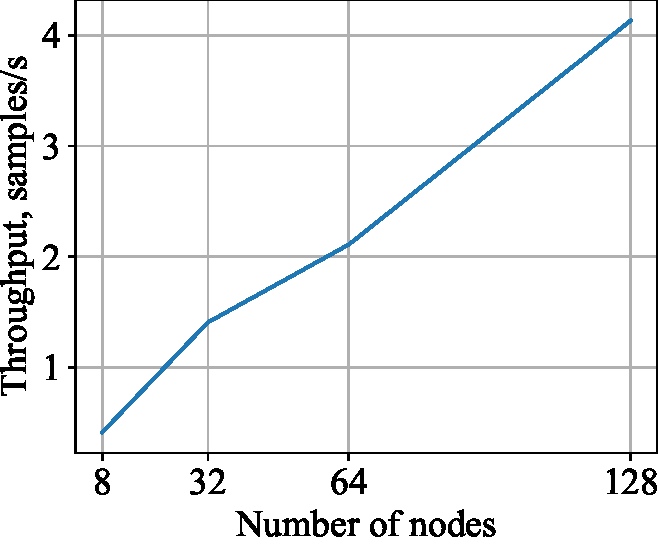
\includegraphics[width=0.7\linewidth]{resources/scaling_t4.pdf}
    \caption{Scaling of SWARM parallelism throughput with the number of nodes.}
    \label{fig:scaling_t4}
\end{figure}


Figure~\ref{fig:scaling_t4} shows the results of our evaluation. It can be seen that the training performance exhibits an approximately linear scaling pattern, which can be explained by the high efficiency of both the stochastic wiring strategy and the auxiliary training components such as the DHT and the All-Reduce protocol used for gradient averaging.

\section{Compression-Aware Architectures}\label{appendix:compression}

Since pipeline parallelism has several distinct points of communication, the network overhead can be reduced considerably by reducing the size of data at these communication points. To exploit this, we develop compression-aware architectures that apply extreme compression at these points. We study two distinct communication bottleneck layers: (1) compression through a linear bottleneck layer, and (2) compression through a bottleneck induced by the maxout activation function~\citep{goodfellow2013maxout}. We also study how compressing the activations and gradients at the communication points to 8 bits affects the predictive performance.

\subsection{Description}\label{appendix:compression_detailed}

\paragraph{Fully connected layers (baseline):} Fully connected layers in models such as Transformers consist of a multilayer perceptron with a single hidden layer and a nonlinear activation function. Without biases and with a residual connection~\citep{resnet} from the inputs to the outputs, this can be described as $\text{MLP}(\mathbf{x}, \mathbf{w}_1, \mathbf{w}_2) = \sigma(\mathbf{x}\mathbf{w}_1)\mathbf{w}_2 + \mathbf{x}$,
where $\mathbf{x}\in\mathbb{R}^{b\times s\times m}$, $\mathbf{w}_1\in\mathbb{R}^{m\times h}$, $\mathbf{w}_2\in\mathbb{R}T^{h\times m}$, and $\sigma(\cdot)$ is a nonlinear activation function such as ReLU~\citep{alexnet}; $b$, $s$, $m$, and $h$ are the batch, sequence, model, and hidden dimensions of the neural network. To compress the output of the MLP layer, we want to apply a compression layer between two consecutive stages. For example, if we have 24 layers and 4 stages, we need 3 compression layers at layers 6, 12, and 18.%

\paragraph{Quantized activations:} A natural way to reduce the communication intensity is to send activations and gradients with respect to activations in reduced precision. However, simply casting tensors to a lower precision may slow down convergence and cause instabilities. Instead, we use dynamic 8-bit quantization with blockwise scaling from~\citep{adam8bit}. This technique reduces communication by ${\approx} 2$x and ${\approx} 4$x for half and full precision, respectively.

On the other hand, quantizing and dequantizing activations can add compute overhead on every microbatch processed. Our implementation circumvents that overhead by performing quantization asynchronously on the CPU. However, this is not required, as blockwise (de)quantization takes less than 1\% of total computation time: see Appendix~\ref{appendix:time_to_solution} for details.


\paragraph{Bottleneck layers:} We experiment with simple bottleneck layers that work by compressing the output features of the MLP by linear projection:
\begin{gather*}
    \text{Bottleneck}(\mathbf{x}, \mathbf{w}_1, \mathbf{w}_2, \mathbf{w}_c, \mathbf{w}_d) = \\ 
    = \text{LayerNorm}(\text{LayerNorm}(\text{MLP}(\mathbf{x}, \mathbf{w}_1, \mathbf{w}_2))\mathbf{w}_c)\mathbf{w_d},
\end{gather*}

where $\mathbf{w}_c\in\mathbb{R}^{m\times c}$, $\mathbf{w}_d\in\mathbb{R}^{c\times m}$ are compression and decompression parameters with compression dimension $c<m$. We find it critical to use layer normalization \cite{ba2016layernorm} to ensure training without divergence. The parameter matrix $\mathbf{w}_c$ resides in one stage and its outputs are transferred to the next stage that holds the parameters $\mathbf{w}_d$, which requires $m/c$ times less communication compared to the original model. Note that adding a bottleneck only adds two linear layers for the forward pass and decreases the size of MLP activations; thus, its computational overhead is negligible (less than 1\% for typical sizes, see Appendix~\ref{appendix:time_to_solution}).

\paragraph{Maxout compression:} Compared to bottleneck compression, maxout compression works by using the maxout activation function~\citep{goodfellow2013maxout} for compression rather than a linear projection. The maxout function of factor $k$ takes inputs with a hidden dimension of $d$ and reduces this dimension by a factor of $k$ by computing the maximum value for each non-overlapping window of $k$ features. We use maxout compression as follows:
\begin{gather*}
    \text{Maxout}(\mathbf{x}, \mathbf{w}_1, \mathbf{w}_2, \mathbf{w}_d) = \\ \text{LayerNorm}(\text{maxout}_k(\text{LayerNorm}(\text{MLP}(\mathbf{x}, \mathbf{w}_1, \mathbf{w}_2))))\mathbf{w_d},
\end{gather*}

where the output is reduced by a factor of $k$ through the maxout function in the previous stage, and then sent to the next stage which holds the decompression matrix $\mathbf{w}_d{\in}\mathbb{R}^{m/k\times m}$.

    \begin{table*}[h!]
    \centering
    \captionof{table}{Performance of compression methods for a Transformer language model with adaptive inputs on WikiText-103. The asterisk denotes that the difference is not statistically significant.}
    \label{tab:steps_to_22}
    \begin{tabular}{@{}lccccc@{}}
    \toprule
    \multirowcell{2}[-0.5ex][l]{Method} & \multirowcell{2}[-0.5ex]{Ppl after\\ 286K steps} & \multirowcell{2}[-0.5ex]{Steps to\\ppl 22} & \multirowcell{2}[-0.5ex]{Data\\ transfer} & \multicolumn{2}{c}{Extra compute} \\ \cmidrule(l){5-6} 
     & &  &  & Absolute & Relative \\ \midrule
    No compression & 21.02 & 1x & 1x & 0 & None \\
    8-bit compression & 21.13 & $\text{0.97x}^{*}$ & 0.5x & 1.2ms & None \tiny{(overlapped)} \\
    Bottleneck & 21.76 & 1.26x & 0.5x & 1.96ms & $\leq 1\%$ \\
    Maxout & 21.83 & 1.28x & 0.5x & 2.04ms & $\leq 1\%$ \\ \bottomrule
    \end{tabular}
    \end{table*}

\subsection{Evaluating the Speed-Quality Tradeoff}
\label{appendix:compression_tradeoff}

While compression techniques reduce the communication overhead, they might also degrade the perplexity reached in a certain time and the final perplexity after a specific number of steps. To study these tradeoffs, we train a Transformer language model with adaptive inputs~\citep{baevski2019adaptiveinputs} on the WikiText-103 dataset and measure how compression-aware architecture variants affect convergence.

Our setup follows that of~\citep{baevski2019adaptiveinputs} with one difference: we use a sequence length of 2048 instead of 3072 to fit this model into our smaller GPUs.
To measure the time to solution, we look at the number of iterations it takes to converge to the training perplexity of \textbf{22}. We evaluate the baseline model and three compression-aware modifications from Section~\ref{appendix:compression_detailed}: bottleneck, maxout, and block-wise dynamic 8-bit quantization, each with 2 pipeline stages and each a compression factor of 2x.

The results can be seen in Table~\ref{tab:steps_to_22}. We can see that 8-bit compression does not degrade the time to 22 perplexity and maintains close to the final perplexity of the baseline. The compression-aware bottleneck and maxout architectures perform equal to each other, but degrade final perplexity slightly and increase time to a perplexity of 22 by 26--28\%.

Using these results, one can determine which method is optimal for their hardware setup. For instance, training with maxout with 2 pipeline stages needs $28\%$ more steps, but accelerates the communication phase by $2$x. If communication is the limiting factor, using maxout or bottleneck compression layers will offer {\it improved} time to perplexity despite the performance degradation. However, the same two techniques would result in slower training in a setup where network bandwidth is unlimited.

In turn, 8-bit quantization reduces communication cost without slowing down per-iteration convergence, making it a ``safe bet'' for situations where the per-iteration convergence must be preserved.
In our large-scale experiments (Section~\ref{sect:experiments_large}), we opt to using quantization since it was enough to fully saturate the GPUs.
If network bandwidth is still a limiting factor, one can combine quantization with bottleneck or maxout compression to further reduce communication.

\vspace{-6pt}
\subsection{Additional Experiments}\label{appendix:compression_extra}

The additional experiments in this section have two purposes: (1) to evaluate how compression methods vary with the number of stages and (2) to evaluate an additional setting that is closer to modern pretraining setups such as GPT-2/3.

While (1) has further implications for scaling, (2) is helpful to account for confounding factors that might have been overlooked in the main experiments on WikiText-103. The WikiText-103 baseline uses non-BPE vocabulary, a long sequence length, and uses adaptive inputs \citep{baevski2019adaptiveinputs}, all of which are not frequently used in modern pretrained Transformers since GPT-2 \citep{radford2019language}.

\begin{table*}
\centering
\caption{Results of language models trained on the OpenWebText Corpus (OWT). The baseline model has 253M parameters and is trained for 8 GPU-days. We apply bottleneck and maxout compression to our baseline in 2 and 4 stages with a compression factor between 2--4x. PTB=Penn Treebank, 1BW=Billion word corpus.}
\label{tab:compression}
\begin{tabular}{lcccccccc}\toprule
                &        &             & \multicolumn{6}{c}{Validation perplexity}                        \\ \cmidrule{4-9} 
Model                &  Stages & Compression & OWT & LAMBADA & WikiText-2 & WikiText-103 & PTB    & 1BW   \\\midrule
Baseline        &   --      & -- &   19.7     &  86.4     &    56.2   &    35.4    &  133.0   &   80.9   \\\midrule
8-bit Quantization  &  2      & 2x        &     19.6       &   89.1     &    {\bf 56.0    }  & {\bf   35.0 }        &  132.7   &  79.8    \\
Bottleneck        &   2      & 2x        &   {\bf19.5  }      &  87.7 &     56.5      &    35.2  &  {129.8 }   &   79.2   \\
Maxout  &  2      & 2x        &     19.6       &  {\bf 85.4 }     &     56.6      &   35.2        &  {\bf 126.8 }    &  {\bf78.8  }   \\\midrule
8-bit Quantization  &  4      & 2x        &    {\bf 19.7  }     & {\bf  87.9  }   &    {\bf 56.3    }  & {\bf   35.2 }        &  {\bf133.9 }  &  {\bf79.8}    \\
Bottleneck         &  4      & 2x       &   21.7          &   100.0      &   66.4   &    40.0   &  149.6      &     89.5  \\
Maxout            &  4      & 2x       &  21.4           &  { 89.9  }    & {  63.9 }      &  {     39.5}      & {142.1   }    &   {86.2 }   \\\midrule
Bottleneck        &   2      & 4x        &   21.6          &    99.8     &   64.8        &   39.6          &  145.6      &   88.3    \\
Maxout            &   2      & 4x        & {\bf20.5}      &  {\bf 89.6 }     &   {\bf  60.0}      & {\bf    37.1 }       & {\bf 141.7 }     &  {\bf83.5}     \\\midrule
Bottleneck      & 4  &  4x   &  28.9  &   141.6      &  100.2 &  58.1  &   235.5     &   118.3    \\
Maxout            &  4      & 4x       &   {\bf 21.3} &   {\bf 93.5 }    &  {\bf 63.6  }      & {\bf 39.2}           &   {\bf 147.7 }   & {\bf 89.1  } \\\bottomrule   
\end{tabular}%
\end{table*}

\vspace{-6pt}
\paragraph{Experimental setup:}

As a baseline, we train a Transformer language model~\citep{transformer} on the OpenWebText corpus~\citep{gokaslan2019openwebtext}. We use the following hyperparameters: sequence size 512, 16 layers with model dimension 1024, and hidden dimension 4096 for a total of 253M parameters. We use byte pair encoding~\citep{sennrich-etal-2016-neural,radford2019language} with a vocabulary size of 50264 symbols. We do not use dropout or other regularization, since our models underfit. We run these experiments in Fairseq~\citep{Ott2019fairseqAF}.

We test bottleneck and maxout compression for a compression factor of 50\% and 75\% compared to the original size over two and four stages. We look at how using these compression-aware architectures affects the performance compared to the compression that they achieve.
\vspace{-6pt}

\paragraph{Results:} The results of our compression-aware architectures are shown in Table~\ref{tab:compression}. We can see that while the bottleneck architecture is competitive with maxout for a compression factor of 2x with two stages, maxout has better perplexities if more stages or a higher compression ratio is used. The out-of-distribution perplexities vary consistently with the in-distribution perplexity, which suggests compression-aware architectures do not degrade the out-of-distribution performance more than the in-distribution performance. As such, the maxout compression is an effective technique to reduce the bandwidth requirements of pipeline parallel training further.

While the 8-bit blockwise quantization can only compress the activations by a factor of two (16-bit $\rightarrow$ 8-bit), it does not affect the quality as much when compared to the baseline. As such, the 8-bit quantization appears to be a reliable default choice to reduce the communication overhead for pipeline parallelism.

When considered together with the square-cube law for distributed training and SWARM parallelism, compression-aware architectures allow for better scaling of large neural networks trained over preemptible low-bandwidth peers. Thus, compression-aware architectures improve the accessibility and affordability of training large models outside HPC environments.

\vspace{-6pt}

\section{Time To Solution}\label{appendix:time_to_solution}

In this section, we evaluate the compression-aware techniques proposed in Appendix~\ref{appendix:compression_detailed} from a practitioner's point of view. A natural way to compare these techniques is in terms of ``the time to solution'', i.e., the wall-clock time it takes to achieve the desired validation objective.
In practice, this time depends on three main factors: the compression strategy, the distributed training algorithm, and the computational infrastructure.

In order to disentangle these factors, we first address the relationship between the training algorithm and the infrastructure.
As we discuss in Section~\ref{sect:method_swarm} (and later in Appendix~\ref{appendix:equivalence}), SWARM parallelism has the same per-iteration behavior as other synchronous methods. Theoretically, the choice of an optimal training system should come down to whichever algorithm has the highest training throughput.




To verify this argument in practice, we compare the per-iteration and per-hour performance of SWARM against fully synchronous training. For this experiment, we train the ALBERT model~\citep{albert} on the WikiText-103 dataset~\citep{wikitext103}. We use the ALBERT-Large architecture with 4 layer groups that correspond to 4 SWARM stages \textit{without the architecture modifications from Appendix~\ref{appendix:compression}}. We follow the exact hyperparameters from the original paper: for example, we use the LAMB optimizer~\citep{lamb} with the batch size of 4096 and the sequence length of 512. We train this model in three setups: traditional distributed training with 8 V100 workers, SWARM with 8 preemptible V100 GPUs, and SWARM with 32 preemptible T4 workers.

\begin{table}[t]
\centering
\captionof{table}{Training time and costs.}
\label{tab:cost}
\begin{tabular}{@{}lccc@{}}
\toprule
\multirowcell{2}[-0.5ex][l]{Setup} & \multirowcell{2}[-0.5ex]{Time, hours} & \multicolumn{2}{c}{Cost, \$} \\
\cmidrule(lr){3-4} 
    & & Hourly & Total \\
\midrule
$8\times V100$, reliable         &175.4&7.834&1374\\
\midrule
$8\times V100$, preemptible           &192.6&5.383&1037\\
\midrule
$32 \times T4$, preemptible           &140.8&3.536&497.8\\
\bottomrule
\end{tabular}
\end{table}

To quantify the time to solution, we measure the wall time required to achieve the ALBERT objective equal to \textbf{1.5}. Additionally, we report the per-hour cost of each experimental setup and the total cost of achieving a loss of 1.5 using public cloud provider pricing estimates in \cref{tab:cost}.

Figure~\ref{fig:convergence_iterations} demonstrates that SWARM matches the per-iteration learning curves of traditional distributed training (PyTorch DistributedDataParallel) up to the variation comparable to caused by changing the random seed. However, SWARM parallelism can achieve the loss of 1.5 more cost-efficiently and faster by using preemptible instances. In turn, \textit{when forced to use homogeneous and reliable GPUs}, SWARM would have slightly inferior performance compared to conventional algorithms, which was first demonstrated in Section~\ref{appendix:training_throughput}.

\begin{figure}
\centering
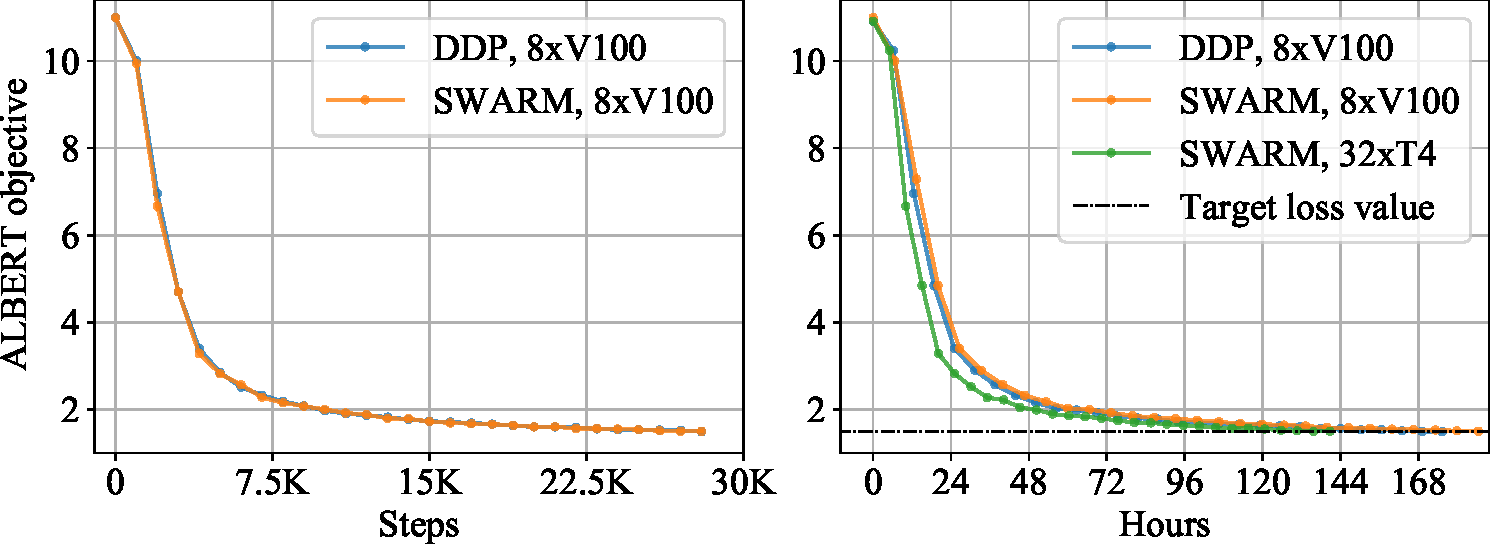
\includegraphics[width=\linewidth]{resources/albert_learning_curves.pdf}
\captionof{figure}{Convergence curves of ALBERT with SWARM and standard data-parallel training.}
\label{fig:convergence_iterations}
\end{figure}

\end{document}
